\chapter{\gkchapter{La syntaxe profonde}{Entre syntaxe et sémantique}}\label{sec:13}

\section{Sémantique, syntaxe profonde, syntaxe de surface}

La \terme{syntaxe profonde} étudie le lien entre le niveau syntaxique et le sens. C’est le contrepoint de la topologie qui s’intéresse au lien entre le niveau syntaxique et le texte.

La structure syntaxique proprement dite, qui décrit comment se combinent les syntaxèmes, est aussi appelée la \terme{structure syntaxique de surface}, par contraste avec la syntaxe profonde. La structure sémantique, et plus précisément la structure prédicative (voir la \sectref{sec:1.2.2} \textit{Partir d’un sens}), décrit les relations prédicat-argument entre les sémantèmes. La syntaxe profonde s’intéresse à la correspondance entre la structure sémantique et la structure syntaxique de surface, c’est-à-dire à l’\terme{interface sémantique-syntaxe}. Cette correspondance est décrite au travers d’une structure qu’on appelle la structure syntaxique profonde.

\Definition{\terme{structure syntaxique profonde}, \terme{relation syntaxique profonde}}
{La \terme{structure syntaxique profonde} d’un énoncé est une structure qui indique comment les \hi{sémantèmes} de cet énoncé \hi{se combinent}. Les \terme{relations syntaxiques profondes} entre les sémantèmes indiquent à la fois la nature de la relation sémantique et de la relation syntaxique entre eux.}

Donnons un premier exemple de structure syntaxique profonde, en la contrastant avec la structure syntaxique de surface et la structure prédicative sémantique (voir la figure \ref{fig:jambe}). 

\ea\label{ex:jambe} \textit{Zoé a tenu la jambe à la prof pendant une heure.}\z

Dans l’exemple \REF{ex:jambe}, \phraseme{tenir la jambe} est un phrasème (voir la \sectref{sec:2.3.7} sur le \textit{Phrasème}) avec le sens de ‘retenir quelqu'un en lui imposant une discussion inopportune’. C’est-à-dire qu'il s'agit d'un sémantème complexe, qui forme un seul nœud dans la structure syntaxique profonde, mais correspond à plusieurs syntaxèmes et donc plusieurs nœuds dans la structure syntaxique de surface. Les conventions utilisées dans la structure syntaxique profonde seront explicitées dans la suite. On notera tout de suite que les articles, qui sont des lexèmes très grammaticalisés, sont considérés comme la réalisation par défaut d’un sémantème de définitude. Rappelons que les signifiés des sémantèmes lexicaux ou lexies sont indiqués entre guillemets simples (‘prof’, ‘tenir la jambe’, …). Les signifiés des sémantèmes grammaticaux ou grammies peuvent être désignés par des termes (singulier, passé, …) ou par des paraphrases (‘un’, ‘avant maintenant’, …). 



\begin{figure}
	\begin{subfigure}[h]{0.66\textwidth}\centering
		\begin{tikzpicture}[>={Triangle[]},
			label distance=0pt,
			node distance=10mm,
			every label/.style={reset shape}]
			
			\begin{scope}[nodes={CircleNode}]
				\node (zoe) [label=below left:{`Zoé'}] {};
				\node (tenirlajambe) [above right=of zoe,label=left:{`tenir la jambe'}] {};
				\node (passe) [above left=of tenirlajambe, label=above left:{passé}] {};
				\node (durer) [above right=of tenirlajambe,label=above right:{`durer'}] {};
				\node (heure) [below right=of durer,label=right:{`heure'}] {};
				\node (singulier0) [above right=of heure,label=right:{singulier}] {};
				\node (indef) [below right=of heure,label=below right:{indéfini}] {};
				\node (prof) [below right=of tenirlajambe,label=right:{`prof'}] {};
				\node (singulier1) [below left=of prof,label=below:{singulier}] {};
				\node (def) [below right=of prof,label=below:{défini}] {};
			\end{scope}
			
			\draw[-{Triangle[]}] (tenirlajambe) -- (zoe) node[font=\footnotesize,midway,anchor=south east, inner sep=1pt] {1};
			\draw[-{Triangle[]}] (durer) -- (tenirlajambe) node[font=\footnotesize,midway,anchor=base east] {1};
			\draw[-{Triangle[]}] (durer) -- (heure) node[font=\footnotesize,midway,anchor=base west] {2};
			\draw[-{Triangle[]}] (passe) -- (tenirlajambe) node[font=\footnotesize,midway,anchor=base west] {1};
			\draw[-{Triangle[]}] (tenirlajambe) -- (prof) node[font=\footnotesize,midway,anchor=base west] {2};
			\draw[-{Triangle[]}] (indef) -- (heure) node[font=\footnotesize,midway,anchor=base west] {1};
			\draw[-{Triangle[]}] (singulier1) -- (prof) node[font=\footnotesize,midway,left] {1};
			\draw[-{Triangle[]}] (def) -- (prof) node[font=\footnotesize,midway,right] {1};
			\draw[-{Triangle[]}] (singulier0) -- (heure) node[font=\footnotesize,midway,anchor=base east] {1};
		\end{tikzpicture}
		\caption{Structure prédicative sémantique}
	\end{subfigure}%
	\bigskip\medskip\\%
	\begin{subfigure}[b]{0.5\textwidth}\centering
		\begin{forest} for tree={font=\normalfont, l sep=6.5mm}
			[\phraseme{tenir le jambe}\textsubscript{passé},calign=child,calign primary child=2
				[\textsc{Zoé},edge label={node[midway,above left=-0.5ex,font=\footnotesize]{1}}]
				[\textsc{prof}\textsubscript{sg,déf},edge label={node[midway,right,font=\footnotesize]{2}}]
				[\textsc{pendant},edge label={node[midway, above right=-0.5ex,font=\footnotesize\itshape]{\textsc{mod}}}
					[\textsc{heure}\textsubscript{sg,indéf},edge label={node[midway,right,font=\footnotesize]{2}}]
				]
			]
		\end{forest}
		\caption{Structure syntaxique profonde}
	\end{subfigure}%
	\hfill
	\begin{subfigure}[b]{0.5\textwidth}\centering
		\begin{forest} for tree={font=\normalfont, l sep=6.5mm}
			[\textsc{avoir}\textsubscript{ind,prés,3,sg}
				[\textsc{Zoé},edge label={node[midway,above left=-1ex,font=\footnotesize]{sujet}}]
				[\textsc{tenir}\textsubscript{part,passé},edge label={node[midway,above right=-1ex,font=\footnotesize]{comp{\NoAutoSpacing :}aux}},calign=child,calign primary child=2
					[\textsc{jambe}\textsubscript{sg},edge label={node[midway, above left=-1ex,font=\footnotesize]{comp{\NoAutoSpacing :}obj}}
						[\textsc{le}\textsubscript{fém,sg},edge label={node[midway,left,font=\footnotesize]{dét}}]
					]
					[\textsc{à},edge label={node[pos=0.75,right=-0.875cm,font=\footnotesize]{comp:obl}}
						[\textsc{prof}\textsubscript{sg},edge label={node[midway,right,font=\footnotesize]{comp}}
							[\textsc{le}\textsubscript{fém,sg},edge label={node[midway,left,font=\footnotesize]{dét}}]
						]
					]
					[\textsc{pendant},edge label={node[midway,above right=-0.5ex,font=\footnotesize]{mod}}
						[\textsc{heure}\textsubscript{sg},edge label={node[midway,right,font=\footnotesize]{comp}}
							[\textsc{un}\textsubscript{fém,sg},edge label={node[midway,left,font=\footnotesize]{dét}}]
						]
					]
				]
			]
		\end{forest}
		\caption{Structure syntaxique de surface}
	\end{subfigure}
\caption{Structures pour \REF{ex:jambe}\label{fig:jambe}}
\end{figure}

On peut voir la structure syntaxique profonde essentiellement comme une \hi{projection de la structure prédicative sur la structure syntaxique de surface} et donc comme une structure syntaxique de surface dont la granularité serait celle des sémantèmes. Néanmoins les relations syntaxiques profondes indiquent à la fois les connexions syntaxiques et les relations prédicat-argument, qui peuvent, dans certains cas, ne pas se superposer aux connexions syntaxiques.

On peut aussi voir la structure syntaxique profonde, à l’inverse, comme une projection de la structure syntaxique sur la structure prédicative, c’est-à-dire comme une \hi{structure sémantique hiérarchisée}. La structure syntaxique profonde se distingue néanmoins de la structure sémantique par la nature des unités en jeu : si la structure sémantique représente a priori un sens et donc la combinaison des signifiés des sémantèmes, la structure syntaxique profonde représente la combinaison des sémantèmes proprement dits, c’est-à-dire d’unités lexicales et grammaticales. Nous allons préciser ce point dans la section suivante.

\chevalier[sec:13-historique]{Historique de la notion de syntaxe profonde}
{La distinction entre syntaxe profonde et syntaxe de surface telle que nous la concevons est due aux travaux d’Igor Mel’čuk dans le cadre de la Théorie Sens-Texte . Pour Mel’čuk, la structure syntaxique profonde est une structure intermédiaire entre la structure sémantique et la structure syntaxique de surface. Dans son cadre théorique (voir l’\encadref{sec:1.3.9} sur \textit{La Théorie Sens-Texte}), le passage du sens au texte est modélisé par un premier ensemble de règles qui transforme la structure sémantique, laquelle comprend les relations prédicat-argument entre signifiés lexicaux, en une structure syntaxique profonde arborescente, qui est ensuite transformée en la structure syntaxique de surface. Plutôt qu’une structure intermédiaire, nous préférons voir la structure syntaxique profonde comme un témoin de la correspondance entre la structure sémantique et la structure syntaxique de surface (voir l’\encadref{sec:13-derivation} sur \textit{Lexique syntaxique et interface sémantique-syntaxe}). 

L’idée d’une structure syntaxique profonde, appelée \terme{structure tectogrammaticale} (voir l’\encadref{sec:13-derivation} pour l’origine du terme), est également présente dans les travaux des Pragois réunis autour de Petr Sgall, qui est l’un des premiers, si ce n’est le premier linguiste (voir son article de \citeyear{sgall1967functional}), à défendre l’idée d’un modèle stratifié des langues, avec différents niveaux de représentation en correspondance les uns avec les autres. On retrouve également un niveau de représentation profond dans un des modèles post-générativistes, la \textit{Lexical Functional Grammar} (LFG) de Ronald Kaplan et Joan Bresnan (\citeyear{kaplan1981lexical}) : ici une structure syntaxique en constituants, la c\textit{-structure}, encode la syntaxe de surface et est opposée à une structure de dépendance dite \terme{structure fonctionnelle}, la f\textit{-structure}, qui s’apparente à une structure syntaxique profonde.

L’opposition terminologique entre structure profonde (\textit{deep structure}) et structure de surface (\textit{surface structure}) a également été utilisée par Noam  \citet{chomsky1965aspects} dans le cadre de la grammaire générative-transformationnelle. L’usage est différent : la structure profonde n’est pas réellement un niveau de représentation différent de la structure de surface, mais une structure syntaxique sous-jacente à la structure de surface, la structure de surface étant obtenue par l’application (éventuelle) de transformations sur la structure profonde. Alors que la structure profonde de Mel’čuk est clairement une structure qui manipule des sémantèmes et pas des syntaxèmes, la structure profonde de Chomsky manipule les mêmes unités que sa structure de surface. De plus, chez Mel’čuk, la structure syntaxique profonde est un arbre de dépendance non ordonnée, l’ordre linéaire n’étant introduit qu’au moment de l’interface entre la syntaxe de surface et le texte, tandis que chez Chomsky, la structure profonde et la structure de surface sont des structures de constituants ordonnées. Il s’ensuit des discussions théoriques, qui nous semblent sans fondement, sur l’\hi{ordre de base} des constructions syntaxiques, l’ordre de base étant l’ordre dans lequel les éléments se trouvent dans la structure profonde avant que des transformations ne les déplacent vers leur position en surface (voir l’\encadref{sec:3.5.8} sur \textit{Mouvement et ordre de base}).}

\section{Argument, actant et modifieur}\label{sec:13-actant}
Les \hi{relations syntaxiques de surface} comme les \hi{relations sémantiques} sont \hi{asymétriques} : les relations syntaxiques de surface lient un gouverneur à un dépendant, tandis que les relations sémantiques lient un prédicat à un argument. Cette \hi{double asymétrie} entraîne qu’il existe deux grands types de \terme{relations syntaxiques profondes} (voir les figures \ref{fig:dep-actant} et \ref{fig:dep-mod} du \chapref{sec:1.2} \textit{Produire un énoncé}).

\Definition{\terme{relation actancielle}, \terme{actant}}
{La relation entre deux sémantèmes est dite \terme{actancielle} quand l’un des sémantèmes est \hi{à la fois le dépendant syntaxique et l’argument sémantique} de l’autre sémantème. Le sémantème dépendant est appelé un \terme{actant} du sémantème gouverneur.}

\Definition{\terme{relation modificative}, \terme{modifieur}}
{La relation entre deux sémantèmes est dite \terme{modificative} quand l’un des sémantèmes est \hi{à la fois le gouverneur syntaxique et l’argument sémantique} de l’autre sémantème. Le sémantème dépendant est appelé un \terme{modifieur} du sémantème gouverneur.}

Le terme \textit{modifieur} est également utilisé pour désigner les sémantèmes qui ont la capacité de modifier un autre sémantème. Nous dirons ainsi que les adjectifs, les adverbes, les prépositions et les conjonctions de subordination sont des modifieurs.

Les relations modificatives sont étiquetées \textsc{mod} dans les structures syntaxiques profondes. Les relations actancielles sont numérotées dans l’\terme{ordre d’oblicité} croissante. L’ordre d’oblicité et son inverse, l’\terme{ordre de saillance}, seront définis dans le \chapfuturef{17}. Disons ici que plus une relation a de «~bonnes~» propriétés, plus elle est saillante : le sujet est la relation la plus saillante, suivie du complément d’objet direct, puis du complément d’objet indirect et des compléments obliques. Le sujet est donc le premier actant du verbe. Pour les modifieurs, le gouverneur syntaxique est considéré comme le premier «~actant~» : ce n'est pas à proprement parler un actant (puisque ce n'est pas un dépendant syntaxique), mais nous nous permettons cet abus de langage car, lorsqu’un modifieur est «~verbalisé~», son gouverneur devient le sujet de la construction (\textit{une \underline{maison} \textbf{verte}}, \textit{la \underline{maison} \textbf{est verte}}). L'actant le plus saillant d'un modifieur (comme \textit{(une personne) heureuse \textbf{de sa réussite}}) est donc appelé son deuxième actant.\largerpage

Nous n'avons pas encore donné de définition de ce qu'est un argument d'un sémantème. Nous tenterons de le faire dans la \sectref{sec:13-argument} sur la \textit{Structure prédicative des sémantèmes}. Nous allons nous intéresser ici un peu plus à la relation entre arguments et actants. Les arguments d'un sémantème sont numérotés en fonction de sa diathèse de base.

\Definition{\terme{diathèse}, \terme{diathèse de base}}
{La \terme{diathèse} d'un sémantème dans un énoncé donné est la correspondance entre les arguments du sémantème et leurs positions syntaxiques dans l'énoncé. On peut généralement déterminer, pour chaque sémantème, une \terme{diathèse de base}, qui correspond à la construction la plus courante et la moins marquée dans la langue.}

En français, un verbe transitif possède deux diathèses principales : la \terme{diathèse active}, où l'agent est réalisé comme sujet, comme en (\ref{ex:13-diathese})a,  et la diathèse passive où c'est le patient, comme en (\ref{ex:13-diathese})b.

\ea\label{ex:13-diathese}
\ea \textit{Un chien poursuit Zoé.}
\ex \textit{Zoé est poursuivie par un chien.}\z\z

La diathèse active est la diathèse de base en français pour les verbes, puisqu'elle est plus courante et nettement moins marquée que la diathèse passive, qui recourt, elle, à un auxiliaire et une préposition. C'est donc l'agent qui sera le premier argument d'un verbe transitif en français et le patient le deuxième argument. (Voir le \chapfuturef{17} pour une discussion plus approfondie sur les notions de sujet, d'agent, et de patient et le cas des langues ergatives, où la diathèse passive peut être la diathèse de base.)

\Definition{\terme{redistribution}, \terme{voix}}
{On appelle \terme{redistribution} toute construction qui suppose un changement de diathèse par rapport à la diathèse de base. On appelle \terme{voix} les grammies qui ont pour unique signification le marquage de la diathèse.}

La grammie qui marque la diathèse passive (en français, \textsc{être} + V\textsubscript{part-passé}) est appelée la \terme{voix passive} ou plus simplement le \terme{passif}. Nous y reviendrons à la \sectref{sec:13-potentiel}. Le passif est en français une redistribution : le premier actant de la diathèse passive est le deuxième argument du verbe.

Les relations actancielles et modificatives ne sont pas les seules relations syntaxiques profondes.
Nous verrons dans la suite (et notamment dans la \sectref{sec:13-controle} et les suivantes) qu’il existe des cas où les relations syntaxiques de surface et les relations sémantiques ne se superposent pas, ce qui nous amènera à considérer deux autres types de relations syntaxiques profondes, que nous appellerons par abus de langage, les \terme{relations syntaxiques pures} et les \terme{relations sémantiques pures} (bien qu'il s'agisse de relations syntaxiques profondes).

Les structures syntaxiques profondes contiennent également des relations de coréférence et des relations d’ancrage, dont nous discuterons dans la \sectref{sec:13-unites} et l’\encadref{sec:13-ancrage}.

Lorsque nous étudierons les listes paradigmatiques (\chapfuturef{18}) et la macrosyntaxe (\chapfuturef{20}), nous introduirons encore d’autres relations syntaxiques profondes.

\section{Les unités (potentielles) de la syntaxe profonde}
\label{sec:13-unites}
L’objectif de la syntaxe profonde est d’étudier les combinaisons entre sémantèmes, c’est-à-dire les unités lexicales et grammaticales qui ont une contribution sémantique. Les unités de base de la structure syntaxique profonde sont donc avant tout les sémantèmes. Mais plusieurs questions se posent et nous allons donc passer en revue les unités qui se trouvent nécessairement dans la structure, celles qui n’y apparaissent pas explicitement et celles qui pourraient y apparaître.

\subsection{Les unités de la syntaxe profonde}

\subsubsection{Les sémantèmes lexicaux} 
Ce sont les \hi{unités lexicales} ou \hi{lexies}. Les lexies peuvent correspondre, du coté syntaxique, à un lexème ou à un phrasème composé de plusieurs lexèmes, comme \phraseme{tenir la jambe} dans l’exemple \REF{ex:jambe}. Elles peuvent éventuellement contenir des grammèmes, comme la lexie \textsc{travaux} (\textit{Il y a des \textbf{travaux} dans ma rue.}), qui contient un pluriel inhérent (ce sens de \textsc{travaux} n'existe pas au singulier; il serait inapproprié de dire \textsuperscript{\#}\textit{Il y a un travail dans ma rue.}).

\begin{sloppypar}
Du côté sémantique, les lexies ont un signifié bien déterminé et sont donc des unités non ambiguës, qui sont associées à des acceptions précises de lexèmes. (Dans nos représentations, nous n’indiquons pas quelle acception de chaque unité lexicale est considérée, car cela nécessite d’avoir un lexique de référence qui attribue un numéro à chaque acceptation.)
\end{sloppypar}

\subsubsection{Les sémantèmes grammaticaux} 
\begin{sloppypar}
Ce sont les \hi{unités grammaticales} ou \hi{grammies}. Une grammie peut correspondre du coté syntaxique à un grammème, comme l’imparfait, ou à une combinaison de grammèmes et de lexèmes, l’un des grammèmes se combinant avec un lexème ne faisant pas partie de la grammie. Ce dernier cas peut être illustré par l’accompli, formé en français d’un auxiliaire, \textsc{avoir} ou \textsc{être}, et d’un grammème de participe passé (voir la figure \ref{fig:accompli}).
\end{sloppypar}

\ea\label{ex:accompli} \textit{J’ai peur d’avoir répondu trop vite.}\z
\begin{figure}
\begin{forest} for tree={font=\normalfont}
	[\phraseme{avoir peur}\textsubscript{présent}
		[\textsc{moi},edge label={node[midway,above left=-0.5ex,font=\footnotesize]{1}}]
		[\textsc{répondre}\textsubscript{accompli},edge label={node[midway, above right=-0.5ex,font=\footnotesize]{2}}
			[\textsc{vite},edge label={node[midway, right,font=\footnotesize\itshape]{\textsc{mod}}}
				[\textsc{trop},edge label={node[midway, right,font=\footnotesize\itshape]{\textsc{mod}}}]
			]			
		]
	]
\end{forest}
\caption{Structure syntaxique profonde de \REF{ex:accompli}\label{fig:accompli}}
\end{figure}

\noindent (Il existe une autre acception de \textit{avoir peur} qui est une collocation, où \textsc{peur} est modifiable et \textit{avoir} commute avec \textsc{faire} : \textit{j’ai une peur bleue des araignées}. Mais le sens figuré, sans déterminant, utilisé en \REF{ex:accompli} est bien un phrasème \phraseme{avoir peur}.)

\subsection{Les unités de la syntaxe de surface qui ne sont pas des unités de la syntaxe profonde}

\subsubsection{Les lexèmes polysémiques}
Nous avons défini les syntaxèmes sur des critères purement syntaxiques. Un lexème, c’est-à-dire un syntaxème lexical, peut tout à fait être polysémique et correspondre à plusieurs sémantèmes. Dans ce cas, c’est une acception précise du lexème, correspondant à un sens particulier, qui figure dans la structure syntaxique profonde. Autrement dit, en analyse, la désambiguïsation lexicale se fait dans le passage de la syntaxe de surface à la sémantique.

\subsubsection{Les lexèmes qui font partie d’un phrasème} 
Dans ce cas, le lexème n’apparaît pas en tant que tel : c’est le phrasème qui sera une unité minimale de la structure syntaxique profonde, comme \phraseme{avoir peur} dans la figure \ref{fig:accompli}.

\subsubsection{Les régimes}
Les syntaxèmes qui marquent la relation syntaxique entre deux sémantèmes n’apparaissent pas explicitement dans la structure syntaxique profonde. Ils ne correspondent pas à un choix séparé du locuteur, mais sont imposés par le régime du gouverneur. C’est le cas de la préposition \textsc{à} dans l’exemple \REF{ex:jambe}, qui est imposé par le régime de \phraseme{tenir la jambe}. C’est aussi le cas des syntaxèmes flexionnels de cas, comme le nominatif porté par les pronoms personnel sujet en français (cf. je = \textsc{moi}\textsubscript{nominatif}, dans l’exemple \REF{ex:accompli}).

\subsubsection{Les syntaxèmes d’accord} 
Les syntaxèmes flexionnels qui marquent l’accord, comme l’accord en genre des adjectifs du français (\textit{maison blanch\textbf{e}}), n’ont pas de contribution sémantique. Ces syntaxèmes servent généralement à marquer des relations syntaxiques. Le cas de l’accord en nombre entre le nom et l’article (\textit{l\textbf{es} chev\textbf{aux}}) est plus complexe, car il y a bien un sémantème de pluriel, qui correspond à deux syntaxèmes (voir l’\encadref{sec:2.3.4} «~\textit{Constructions verbales et accords : signes vides ?}~».) Nous positionnons le sémantème sur le nom, puisque c’est sur le nom que porte sémantiquement le nombre (même si en français, le nombre est morphologiquement marqué avant tout sur l’article).

\subsection{Les unités potentielles de la syntaxe profonde}\label{sec:13-potentiel}

\subsubsection{Les fonctions lexicales pour les collocatifs}
Les collocatifs sont des sémantèmes, mais leur choix est contraint par la base de la collocation et leur sens dans le contexte de la collocation est généralement différent de leur sens habituel. Dans l’exemple \REF{ex:peurbleue}, \textsc{faire} et \textsc{bleu} sont des collocatifs de \textsc{peur}, qui expriment respectivement des sens de causation (‘Zoé cause que j’ai peur’) et d’intensification (‘Ma peur est intense’), auxquels nous assignons les signifiés génériques ‘causer’ et ‘intense’ dans la représentation sémantique de la figure \ref{fig:peurbleue}a. À partir de là deux choix sont possibles : on peut introduire des lexies \textsc{faire} et \textsc{bleu} particulières, utilisées avec les sens ‘causer’ et ‘intense’ dans le contexte de \textsc{peur}. Ou bien, comme le propose Igor Mel’čuk, considérer que \textsc{faire} et \textsc{bleu} sont des lexèmes qui réalisent en surface les valeurs d’un «~sémantème~» plus abstrait, qu’il appelle des \terme{fonctions lexicales} (voir l'\encadref{sec:2.3.11} sur les \textit{Fonctions lexicales}) et que nous nommons Caus et Magn dans la figure \ref{fig:peurbleue}b (voir la \sectref{sec:13-controle} sur le \textit{Contrôle} pour la flèche hachée).

\ea\label{ex:peurbleue} \textit{Zoé m’a fait une peur bleue.}\z

\begin{figure}
	\begin{subfigure}[b]{0.5\textwidth}
		\begin{tikzpicture}[>={Triangle[]},
			label distance=0pt,
			node distance=10mm,
			every label/.style={reset shape}]
			
			\begin{scope}[nodes={CircleNode}]
				\node (zoe) [label=below left:{`Zoé'}] {};
				\node (causer) [above right=of zoe,label=above:{`causer'}] {};
				\node (peur) [below right=of causer,label=below left:{`peur'}] {};
				\node (intense) [above right=of peur,label=above:{`intense'}] {};
				\node (moi) [below right=of peur,label=below right:{`moi'}] {};
			\end{scope}
			
			\draw[-{Triangle[]}] (causer) -- (zoe) node[font=\footnotesize,midway,anchor=base east] {1};
			\draw[-{Triangle[]}] (causer) -- (peur) node[font=\footnotesize,midway,anchor=base west] {2};
			\draw[-{Triangle[]}] (intense) -- (peur) node[font=\footnotesize,midway,anchor=base east] {1};
			\draw[-{Triangle[]}] (peur) -- (moi) node[font=\footnotesize,midway,anchor=base west] {1};
			
		\end{tikzpicture}
		\caption{Structure prédicative sémantique}
	\end{subfigure}%
	\hfill
	\begin{subfigure}[b]{0.5\textwidth}
		\centering
		\begin{forest} for tree={font=\normalfont}
			[Caus\textsubscript{passé}
			[\textsc{Zoé},edge label={node[midway,above left=-0.5ex,font=\footnotesize]{1}}]
			[\textsc{peur},name=peur,edge label={node[midway,right,font=\footnotesize]{2}}
			[Magn,edge label={node[midway,left,font=\footnotesize\itshape]{\textsc{mod}}}]
			]
			[\textsc{moi},name=moi,edge label={node[midway,above right=-0.5ex,font=\footnotesize]{3}}]
			]
			\draw[->,dashed] ($(peur)+(0.125cm,-0.4cm)$) .. controls +(south:0.6cm) and +(south:1cm) .. (moi) node[pos=0.5,below right]{\footnotesize 1};
		\end{forest}
		\caption{Structure syntaxique profonde}
	\end{subfigure}
\caption{Structures avec fonctions lexicales de \REF{ex:peurbleue}\label{fig:peurbleue}}
\end{figure}

\subsubsection{Les translatifs purs} 
Les \terme{translatifs} sont des syntaxèmes dont la fonction est de permettre à un lexème d’une catégorie donnée d’occuper une position syntaxique dont les éléments prototypiques appartiennent à une autre catégorie (voir le \chapfuturef{16} sur les \textit{Catégories microsyntaxiques}). Ainsi dans l’exemple (\ref{ex:sympa})a, la copule \textsc{être} permet à l’adjectif \textsc{sympa} de se comporter comme un prédicat verbal et d’occuper la position de complément du verbe \textsc{penser}. Une autre construction est possible, (\ref{ex:sympa})b, sans copule, et la synonymie entre les deux constructions montre l’absence de contribution sémantique de la copule. Un translatif sans réelle contribution sémantique est dit \terme{pur}.

\ea\label{ex:sympa}
    \ea \textit{Ali trouve que Zoé est sympa.}
\ex \textit{Ali trouve Zoé sympa.}\z\z

Malgré l’absence de contribution sémantique des translatifs purs, nous décidons de les faire figurer dans la structure syntaxique profonde, car on peut considérer que le fait de ne pas utiliser, dans une position donnée, une lexie de la catégorie attendue est un choix du locuteur (souvent contraint par l’absence d’une possible réalisation dans la catégorie attendue du sens à lexicaliser) et que ce choix induit une lexicalisation particulière dans la position considérée. De plus, dans un cas comme celui de \textsc{sympa} dans (\ref{ex:sympa})a, le fait que l’adjectif soit combiné avec un translatif en verbe entraîne la présence d’une grammie de temps, le présent dans cet exemple, dont le choix est en partie libre. 
Il existe plusieurs possibilités pour modéliser la copule dans la structure syntaxique profonde de (\ref{ex:sympa})a. Dans la figure \ref{fig:sympa}a, nous représentons la copule comme un opérateur V de verbalisation, tandis que, dans la figure  \ref{fig:sympa}b, nous lui attribuons une véritable position dans la structure (ce qui nous rapproche davantage de la structure syntaxique de surface). Dans ce deuxième cas, nous utilisons l’étiquette Pred, comme ‘prédicatif’, comme le propose Mel’čuk. La flèche hachée représente une dépendance sémantique qui n’est pas réalisée par une dépendance syntaxique entre les mêmes éléments. Nous y reviendrons dans la \sectref{sec:13-controle} sur le \textit{Contrôle}.

\begin{figure}
	\begin{subfigure}[b]{0.5\textwidth}
		\centering
		\begin{forest} for tree={font=\normalfont}
			[\textsc{trouver}\textsubscript{prés}
				[\textsc{Ali},edge label={node[midway,above left=-0.5ex,font=\footnotesize]{1}}]
				[V(\textsc{sympa})\textsubscript{prés},edge label={node[midway,above right=-0.5ex,font=\footnotesize]{2}}
					[\textsc{Zoé},edge label={node[midway,right,font=\footnotesize]{1}}]
				]
			]
		\end{forest}
		\caption{Avec la copule comme opérateur}
	\end{subfigure}%
	\hfill
	\begin{subfigure}[b]{0.5\textwidth}
		\centering
		\begin{forest} for tree={font=\normalfont}
			[\textsc{trouver}\textsubscript{prés}
				[\textsc{Ali},edge label={node[midway,above left=-0.5ex,font=\footnotesize]{1}}]
				[Pred\textsubscript{prés},edge label={node[midway,above right=-0.5ex,font=\footnotesize]{2}}
					[\textsc{Zoé},name=zoe,edge label={node[midway,above left=-0.5ex,font=\footnotesize]{1}}]
					[\textsc{sympa},name=sympa,edge label={node[midway,above right=-0.5ex,font=\footnotesize]{2}}]
				]
			]
			\draw[->,dashed] (sympa) to[out=south,in=south] node[pos=0.5,below]{\footnotesize 1} (zoe);
		\end{forest}
		\caption{Avec un nœud lexical pour la copule}
	\end{subfigure}
\caption{Deux représentations pour la structure syntaxique profonde de (\ref{ex:sympa})a avec une copule\label{fig:sympa}}
\end{figure}

Notons que la conjonction de subordination \textsc{que} est également un translatif pur (de verbe en substantif). Nous aurions donc pu aussi l’introduire dans les représentations de la figure \ref{fig:sympa}. Nous ne l’avons pas fait, car on considère que la conjonction de subordination \textsc{que} fait partie du régime de \textsc{trouver}.

Notons également que les translatifs peuvent en plus être des collocatifs : tel est le cas des verbes supports qui permettent à des noms prédicatifs d’occuper des positions verbales (\textit{\textbf{poser} une question}, \textit{\textbf{faire} une sieste}, \textit{\textbf{pousser} un cri}, etc. (voir l’\encadref{sec:2.3.9} sur les \textit{Verbes supports et unités grammaticales}).

\subsubsection{Les sémantèmes constructionnels} 
Il existe des syntaxèmes qui n’expriment pas des sens proprement dits, mais qui ont à voir avec la structure communicative, la façon dont on présente l’information (voir l’\encadref{sec:13-packaging}). Nous considérons qu’il s’agit de sémantèmes d’un type particulier, que nous appelons les \terme{sémantèmes constructionnels}. Nous distinguons ceux comme le clivage, qui sont réalisés par des lexèmes et des grammèmes distincts de la forme verbale et que nous traitons comme des lexies, et ceux comme le passif, qui sont réalisés par un grammème sur le verbe et que nous traitons comme des grammies.

Nous avons déjà parlé du clivage dans la \sectref{sec:3.4.10} sur \textit{Les tests de constituance} et dont nous reparlerons dans le \chapfuturef{19}. Le clivage, réalisé par \textit{c’est} X \textit{qui/que} Y, s’applique à une proposition Y dont il promeut l’un des éléments X. Il possède donc deux actants : l’élément promu X est le premier actant et la proposition Y privée de cet élément est le deuxième actant.

\ea\label{ex:13-clivage}
\ea \textit{\textbf{C’est} Zoé \textbf{qui} viendra.}
\ex \textit{\textbf{C’est} à Zoé \textbf{que} j’ai parlé.}\z\z
Nous modélisons le clivage comme une lexie que nous appelons « clivage ». Les structures syntaxiques profondes des exemples \REF{ex:13-clivage} sont données dans la figure \ref{fig:13-clivage}.

\begin{figure}
	\begin{subfigure}[b]{0.5\textwidth}
		\centering
		\begin{forest} for tree={font=\normalfont}
			[clivage
			[\textsc{Zoé},name=zoe,edge label={node[midway,above left=-0.5ex,font=\footnotesize]{1}}]
			[\textsc{venir}\textsubscript{futur},name=venir,edge label={node[midway,above right=-0.5ex,font=\footnotesize]{2}}]
			]
			\draw[->,dashed] (venir) to[out=south,in=south] node[pos=0.5,below]{\footnotesize 1} (zoe);
		\end{forest}
		\caption{Structure de (\ref{ex:13-clivage})a}
	\end{subfigure}%
	\hfill
	\begin{subfigure}[b]{0.5\textwidth}
		\centering
		\begin{forest} for tree={font=\normalfont}
			[clivage
			[\textsc{Zoé},name=zoe,edge label={node[midway,above left=-0.5ex,font=\footnotesize]{1}}]
			[\textsc{parler}\textsubscript{passé},name=parler,edge label={node[midway,above right=-0.5ex,font=\footnotesize]{2}}
			[\textsc{moi},edge label={node[midway,right,font=\footnotesize]{1}}]
			]
			]
			\draw[->,dashed] ($(parler)+(-0.125cm,-0.4cm)$) .. controls +(south:0.6cm) and +(south:1cm) .. (zoe) node[pos=0.5,below]{\footnotesize 2};
		\end{forest}
		\caption{Structure de (\ref{ex:13-clivage})b}
	\end{subfigure}
\caption{Structures syntaxiques profondes pour le clivage\label{fig:13-clivage}}
\end{figure}

Passons à notre deuxième exemple de sémantème constructionnel, le passif. Il s'agit d'une redistribution qui a pour effet de promouvoir l’objet d’un verbe transitif dans la position sujet et d’effacer ou de rétrograder le sujet du verbe. En français, il est réalisé par un grammème de participe passé sur le verbe, généralement combiné avec la copule \textsc{être}. En conséquence de cette redistribution, le deuxième argument du verbe devient le premier actant, tandis que le premier argument est rétrogradé dans un rôle que nous notons ∞. (Nous utilisons cet étiquette pour indiquer que le \terme{complément rétrogradé}, appelé \terme{complément d’agent} par la grammaire traditionnelle, occupe toujours une position plus oblique que les autres actants. Nous y reviendrons lorsque nous parlerons du causatif dans la \sectref{sec:13-montee}.)

\ea\label{ex:13-passif}
\ea \textit{une fille poursuivie par un chien}
\ex \textit{Zoé est poursuivie par un chien.}\z\z

\begin{figure}
	\begin{subfigure}[b]{0.5\textwidth}
		\centering
		\begin{forest} for tree={font=\normalfont}
			[\textsc{fille}\textsubscript{sg,indéf}
				[\textsc{poursuivre}\textsubscript{passif},edge label={node[midway,right,font=\footnotesize\itshape]{\textsc{mod}}}
					[\textsc{chien}\textsubscript{sg,indéf},edge label={node[midway,right,font=\footnotesize]{$\infty$}}]
				]
			]
		\end{forest}
		\caption{Structure de (\ref{ex:13-passif})a}
	\end{subfigure}%
	\hfill
	\begin{subfigure}[b]{0.5\textwidth}
		\centering
		\begin{forest} for tree={font=\normalfont}
			[V(\textsc{poursuivre}\textsubscript{passif})\textsubscript{prés}
				[\textsc{Zoé},edge label={node[midway,above left=-0.5ex,font=\footnotesize]{1}}]
				[\textsc{chien}\textsubscript{sg,indéf},edge label={node[midway,above right=-0.5ex,font=\footnotesize]{$\infty$}}]
			]
		\end{forest}
		\caption{Structure de (\ref{ex:13-passif})b}
	\end{subfigure}
\caption{Structures syntaxiques profondes pour le passif\label{fig:13-passif}}
\end{figure}

Nous faisons le choix de traiter le passif complet en \textsc{être} + V\textsubscript{part-passé} comme la combinaison d'une grammie que nous appelons le passif et qui est réalisée par le grammème du participe passé, comme en \REF{ex:13-passif}a, et d'une translation d'adjectif en verbe réalisée par la copule \textsc{être}. La grammie du passif assure, elle, une translation du verbe en adjectif, puisque le participe passif peut modifier un nom, et une redistribution, puisque le deuxième actant du verbe est promu comme gouverneur et le premier actant est rétrogradé. Dans la figure \ref{fig:13-passif}a, nous notons cette grammie «~passif~», mais il est aussi possible de la noter Adj\textsubscript{2}, c'est-à-dire comme la réalisation d'une translation en adjectif promouvant le deuxième actant. Les notations \textsc{poursuivre}\textsubscript{passif} et Adj\textsubscript{2}(\textsc{poursuivre}) sont donc à peu près équivalentes, la deuxième notation étant plus générale. Le passif en \textsc{être} est analysée comme une double translation, du verbe en adjectif par la grammie du passif, puis d’adjectif en verbe par la copule (voir la figure \ref{fig:13-passif}b).

En français, la valence active est la valence de base du verbe et cette valence n'est pas marquée, la forme du verbe étant la même que celle des verbes intransitifs.  Nous considérons, en conséquence, qu'il n'y a pas de grammie de l'actif.

\subsubsection{Les pronoms}
Certains pronoms résultent du dédoublement d’un nœud sémantique, comme le pronom \textit{elle} en (\ref{ex:13-pronom})a. Le pronom n’est donc pas un sémantème standard, puisqu’il n’a pas de signifié distinct qui apparaisse dans la structure sémantique, comme on le voit dans la structure prédicative de la figure \ref{fig:13-pronom-sem} commune aux deux exemples en \REF{ex:13-pronom}.

\ea\label{ex:13-pronom}
\ea \textit{Zoé pense qu’elle viendra}.
\ex \textit{Zoé pense venir}.\z\z

\begin{figure}
\begin{tikzpicture}[>={Triangle[]},
	label distance=0pt,
	node distance=10mm,
	every label/.style={reset shape}]
	
	\begin{scope}[nodes={CircleNode}]
		\node (zoe) [label=below left:{`Zoé'}] {};
		\node (penser) [above right=of zoe, label=above:{`penser'}] {};
		\node (venir) [below right=of penser, label=below right:{`venir'}] {};
	\end{scope}
	
	\draw[-{Triangle[]}] (penser) -- (zoe) node[font=\footnotesize,midway,,anchor=base east] {1};
	\draw[-{Triangle[]}] (penser) -- (venir) node[font=\footnotesize,midway,,anchor=base west] {2};
	\draw[-{Triangle[]}] (venir) -- (zoe) node[font=\footnotesize,midway,above] {1};
	
\end{tikzpicture}
\caption{Structure prédicative avec un cycle commune à (\ref{ex:13-pronom})a et b\label{fig:13-pronom-sem}}
\end{figure}

La représentation que nous proposons pour (\ref{ex:13-pronom})a est d’indiquer qu’il y a un sémantème « pro » coréférent avec \textsc{Zoé}. La coréférence est indiquée par une flèche bidirectionnelle en pointillé (voir la figure \ref{fig:13-pronom-pro}a). Ce lien indique que le sémantème « pro » provient du dédoublement du sémantème ‘Zoé’ et il permet d’assurer l’accord de « pro » avec \textsc{Zoé} au niveau syntaxique de surface. Dans le cas de (\ref{ex:13-pronom})b, où il n’y a pas de pronom, nous indiquons, dans la figure \ref{fig:13-pronom-pro}b, que la dépendance entre le verbe subordonné et son premier argument est uniquement sémantique (par une flèche hachée, voir la \sectref{sec:13-controle} sur le \textit{Contrôle}).

\begin{figure}
	\begin{subfigure}[b]{0.5\textwidth}
		\centering
		\begin{forest} for tree={font=\normalfont}
			[\textsc{penser}\textsubscript{prés}
			[\textsc{Zoé},name=zoe,edge label={node[midway,above left=-0.5ex,font=\footnotesize]{1}}]
			[\textsc{venir}\textsubscript{futur},edge label={node[midway,above right=-0.5ex,font=\footnotesize]{2}}
			[pro,name=pro,edge label={node[midway,right,font=\footnotesize]{1}}]
			]
			]
			\draw[<->,dotted] (zoe) to[out=south,in=west] node[pos=0.5,below]{} (pro);
		\end{forest}
		\caption{Structure de (\ref{ex:13-pronom})a}
	\end{subfigure}%
	\hfill
	\begin{subfigure}[b]{0.5\textwidth}
		\centering
		\begin{forest} for tree={font=\normalfont}
			[\textsc{penser}\textsubscript{prés}
			[\textsc{Zoé},name=zoe,edge label={node[midway,above left=-0.5ex,font=\footnotesize]{1}}]
			[\textsc{venir},name=venir,edge label={node[midway,above right=-0.5ex,font=\footnotesize]{2}}]
			]
			\draw[->,dashed] (venir) to[out=south,in=south] node[pos=0.5,below]{\footnotesize 1} (zoe);
		\end{forest}
		\caption{Structure de (\ref{ex:13-pronom})b}
	\end{subfigure}
\caption{Structures syntaxiques profondes dans le cas d’un cycle\label{fig:13-pronom-pro}}
\end{figure}

D’autres représentations plus proches de la sémantique ont été proposées : Mel’čuk propose une représentation commune pour les deux phrases de \REF{ex:13-pronom}, avec deux nœuds \textsc{Zoé} lié par un lien de coréférence. Une alternative à cette représentation est de garder un seul nœud \textsc{Zoé} et d’avoir deux gouverneurs syntaxiques pour ce nœud, ce qui donne une structure de dag (\textit{directed acyclic graph}, voir l’\encadref{sec:1.2.3} sur \textit{Graphe et arbre}).

\subsubsection{La finitude-mode} 
On appelle \terme{finitude-mode} la catégorie comprenant les grammèmes indicatif, subjonctif, impératif, infinitif, participe présent et participe passé. À l’exception de l’impératif, ces grammèmes n’ont généralement pas de contribution sémantique. Par exemple, l’indicatif ou l’infinitif sur le verbe \textsc{venir} dans les exemples \REF{ex:13-pronom} est imposé par le verbe \textsc{penser} qui le régit et nous ne le faisons donc pas figurer dans les structures syntaxiques profondes de ces exemples. Cette décision est tout de même discutable, car même si l’indicatif et l’infinitif n’ont pas ici de contribution sémantique, le choix de l’indicatif plutôt que l’infinitif a des conséquences sur la présence d’un sémantème de temps et sur la réalisation d’un pronom.

La question se pose aussi pour l’indicatif sur le verbe principal. Nous considérons que la réalisation d’un verbe à l’indicatif n’est pas réellement un choix du locuteur et ne correspond pas à l’expression d’un sens particulier. Ce n’est pas tout à fait vrai, puisque le choix de l’indicatif (\textit{Tu fais ce que tu veux.}) s’oppose à celui de l’impératif (\textit{Fais ce que tu veux !}) ou du subjonctif (\textit{Qu’il fasse ce qu’il veut !}) et indique qu’il s’agit d’une assertion ou d’une question et pas d’une injonction.

Il existe des cas où l’infinitif possède réellement une contribution sémantique et n’est pas imposé par le régime d’un verbe. C’est par exemple le cas dans l’exemple (\ref{ex:13-fumer})a : la grammie infinitif de \textit{fumer} en position sujet réalise une valeur générique du premier argument de \textsc{fumer}, que l’on peut aussi exprimer en français avec le pronom \textsc{on}, comme le montre la paraphrase avec (\ref{ex:13-fumer})b. 

\ea\label{ex:13-fumer}
\ea \textit{Fumer est dangereux pour la santé.}
\ex \textit{Quand on fume, on met sa santé en danger.}\z\z
\begin{sloppypar}
Nous donnons dans la figure \ref{fig:13-fumer}a les représentations sémantique et syntaxique profonde de \REF{ex:13-fumer}. Nous représentons le sens générique par une étiquette « générique ». Ce sens est exprimé par grammie infinitif dans la structure syntaxique profonde. Notons que l’infinitif n’apparaît pas dans la structure syntaxique profonde quand il ne s’agit pas d’un sémantème comme ici (voir la figure \ref{fig:13-pronom-pro}b).
\end{sloppypar}

\begin{figure}
	\begin{subfigure}[b]{0.5\textwidth}
		\centering
		\begin{tikzpicture}[>={Triangle[]},
			label distance=0pt,
			node distance=10mm,
			every label/.style={reset shape}]
			
			\begin{scope}[nodes={CircleNode}]
				\node (dangereux) [label=above:{`dangereux'\ }] {};
				\node (fumer) [below right=of dangereux,label=below:{`fumer'}] {};
				\node (generique) [above right=of fumer,label=above:{\ générique}] {};
			\end{scope}
			
			\draw[-{Triangle[]}] (dangereux) -- (fumer) node[font=\footnotesize,midway,left] {1};
			\draw[-{Triangle[]}] (fumer) -- (generique) node[font=\footnotesize,midway,right] {1};
			
		\end{tikzpicture}
		\caption{Structure prédicative sémantique}
	\end{subfigure}%
	\hfill
	\begin{subfigure}[b]{0.5\textwidth}
		\centering
		\begin{forest} for tree={font=\normalfont}
			[V(\textsc{dangereux})\textsubscript{prés}
			[\textsc{fumer}\textsubscript{inf},edge label={node[midway,right,font=\footnotesize]{1}}]
			]
		\end{forest}
		\caption{Structure syntaxique profonde}
	\end{subfigure}
\caption{Structures pour \REF{ex:13-fumer}\label{fig:13-fumer}}
\end{figure}

\begin{sloppypar}
Concernant le grammème de participe passé, nous avons déjà donné des exemples  et vu qu’il pouvait faire partie d’une grammie complexe exprimant le passé (\textsc{avoir}\textsubscript{présent} + V\textsubscript{part-passé}) ou l’accompli (\textsc{avoir} + V\textsubscript{part-passé}) ou qu’il pouvait réaliser la grammie du passif (voir la figure \ref{fig:13-passif}).
\end{sloppypar}

Le grammème de participe présent, lui, est utilisé dans deux emplois en français :  comme un translatif pur de verbe en adjectif, comme en (\ref{ex:13-suivant})a, ou comme un translatif de verbe en adverbe dans la grammie complexe \textsc{en} + V\textsubscript{part-présent}, comme en (\ref{ex:13-suivant})b. Comme expliqué dans la \sectref{sec:13-potentiel}, nous traitons les translatifs purs comme des opérateurs dans la structure syntaxique profonde : le participe présent est ainsi représenté par les opérateurs Adj et Adv dans la figure \ref{fig:13-suivant}. Il serait également possible de nommer les grammies correspondantes. Une grammie assurant la translation d'un verbe en adverbe est généralement appelée un gérondif.

\ea\label{ex:13-suivant}  
\ea \textit{un chemin suivant la rivière}
\ex \textit{Ali est allé à la poste en suivant la rivière.}\z\z

\begin{figure}
	\begin{subfigure}[b]{0.5\textwidth}
		\centering
		\begin{forest} for tree={font=\normalfont}
			[\textsc{chemin}\textsubscript{sg,déf}
			[Adj(\textsc{suivre}),edge label={node[midway,right,font=\footnotesize\itshape]{\textsc{mod}}}
			[\textsc{rivière}\textsubscript{sg,déf},edge label={node[midway,right,font=\footnotesize]{2}}]
			]
			]
		\end{forest}
		\caption{Structure de (\ref{ex:13-suivant})a}
	\end{subfigure}%
	\hfill
	\begin{subfigure}[b]{0.5\textwidth}
		\centering
		\begin{forest} for tree={font=\normalfont, l sep=6.5mm}
			[\textsc{aller}\textsubscript{passé},calign=child,calign primary child=2
				[\textsc{Ali},edge label={node[midway,above left=-0.5ex,font=\footnotesize]{1}}]
				[\textsc{poste}\textsubscript{sg,déf},edge label={node[midway,left,font=\footnotesize]{2}}]
				[Adv(\textsc{suivre}),edge label={node[midway,above right=-0.5ex,font=\footnotesize\itshape]{\textsc{mod}}}
					[\textsc{rivière}\textsubscript{sg,déf},edge label={node[midway,right,font=\footnotesize]{2}}]
				]
			]
		\end{forest}
		\caption{Structure de (\ref{ex:13-suivant})b}
	\end{subfigure}
\caption{Structures syntaxiques profondes pour le participe présent\label{fig:13-suivant}}
\end{figure}

\subsubsection{Les sémantèmes cachés}\label{sec:13-cache}
\begin{sloppypar}
Nous appelons \textsc{sémantèmes cachés} des sens qui naissent d’une configuration particulière sans être réellement réalisés par un syntaxème. Notre premier exemple est illustré par une construction particulière du russe relevée par \citet[141]{melcuk1988dependency}. En russe, le numéral se place normalement avant le nom. Il est néanmoins possible de placer le numéral après le nom, mais cela change le sens : le numéral est alors interprété comme une valeur approximative. C’est donc l’ordre des mots qui est signifiant. 
\end{sloppypar}

\ea\label{ex:13-approx}  
\ea \textit{Ja polučil desjat’ rublej.}\\ 
\glt ‘J’ai reçu dix roubles.’
\ex \textit{Ja polučil rublej desjat’.}\\ 
\glt ‘J’ai reçu environ dix roubles.’\z\z
Nous indiquons cette valeur par un sémantème « approx », qui se combine avec le numéral (voir la figure \ref{fig:13-approx}). Plus généralement, nous représentons les sémantèmes cachés comme des sémantèmes opérationnels s’appliquant à un autre sémantème.

\begin{figure}
% FIGURE 11
\begin{forest} for tree={font=\normalfont}
	[\textsc{polučit'}\textsubscript{accompli,passé}
	[\textsc{ja},edge label={node[midway,above left=-0.5ex,font=\footnotesize]{1}}]
	[\textsc{rubl'}\textsubscript{pl},edge label={node[midway,above right=-0.5ex,font=\footnotesize]{2}}
	[approx(\textsc{desjat'}),edge label={node[midway,right,font=\footnotesize\itshape]{\textsc{mod}}}]
	]
	]
\end{forest}
\caption{Structure syntaxique profonde pour le sémantème configurationnel de (\ref{ex:13-approx})b\label{fig:13-approx}}
\end{figure}

La \terme{dislocation}, gauche ou droite, est un cas de sémantème constructionnel, comme le clivage, mais qui, à la différence du clivage, n’a pas vraiment de marqueur lexical : une dislocation met généralement en jeu un pronom qui reprend l’élément disloqué, mais le pronom n’est pas en soi le signifiant d’une dislocation (nous verrons d'ailleurs un cas dans l'\encadref{sec:13-packaging} de dislocation droite sans reprise pronominale).

\ea\label{ex:13-disloc} \textit{Zoé, j’ai l’intention de lui parler.}\z
Nous considérons que les dislocations gauche et droite sont des sémantèmes cachés, que nous notons « disloc-g » ou « disloc-d » (voir la figure \ref{fig:13-disloc}). La contribution sémantique de la dislocation gauche sera discutée dans l'\encadref{sec:13-packaging} et la subtile différence de sens entre dislocations gauche et droite sera étudiée dans le \chapfuturef{20}.


\begin{figure}
% FIGURE 12
\begin{forest} for tree={font=\normalfont}
	[V(\textsc{intention})\textsubscript{prés}
		[\textsc{moi},name=moi,edge label={node[midway,above left=-0.5ex,font=\footnotesize]{1}}]
		[\textsc{parler},name=parler,edge label={node[midway,above right=-0.5ex,font=\footnotesize]{2}}
			[\ \ disloc-g(\textsc{Zoé}),edge label={node[midway,right,font=\footnotesize]{2}}]
		]
	]
	\draw[->,dashed] ($(parler)+(-0.125cm,-0.4cm)$) .. controls +(south:0.6cm) and +(south:1cm) .. (moi) node[pos=0.75,below left]{\footnotesize 1};
\end{forest}
\caption{Structure syntaxique profonde pour la dislocation gauche de \REF{ex:13-disloc}\label{fig:13-disloc}}
\end{figure}

Un dernier exemple de sémantème caché est celui des conversions massif-comptable. Un nom comme \textsc{vin} ou \textsc{sable} est dit \terme{massif}, car on ne compte pas le vin ou le sable et que du vin séparé en deux donne toujours du vin.

\ea\label{ex:13-vin}
\ea \textit{Zoé a bu du vin.}
\ex \textit{Zoé a gouté un bon vin.}\z\z
Dans l’exemple (\ref{ex:13-vin})a, nous considérons que \textsc{vin} ne se combine pas avec une grammie de nombre, car le grammème de singulier ne résulte pas d’un choix et ne s’oppose pas à un grammème de pluriel (voir la figure \ref{fig:13-vin})a. Pour quantifier du vin ou du sable, on doit ajouter un « classifieur » : \textit{deux \textbf{bouteilles} de vin}, \textit{trois \textbf{kilos} de sable}. On peut néanmoins combiner les massifs directement avec des numéraux, mais alors le nom X est interprété comme dénotant un «~type de X~». Nous considérons donc que dans l’exemple (\ref{ex:13-vin})b se cache un sémantème opérationnel, «~type~» (voir la figure \ref{fig:13-vin}b). On notera aussi, dans les exemples \REF{ex:13-vin}, le contraste entre l’indéfini réalisé par \textsc{du} pour les massifs et par \textsc{un} pour les comptables. (L'opposition entre défini et indéfini sera étudiée au \chapfuturef{15}.)


\begin{figure}
% Figure 13
	% a. Zoé <-1- boire\_passé -2-> vin\_indéf
	\begin{subfigure}[b]{0.5\textwidth}
		\centering
		\begin{forest} for tree={font=\normalfont}
			[\textsc{boire}\textsubscript{passé}
				[\textsc{Zoé},edge label={node[midway,above left=-0.5ex,font=\footnotesize]{1}}]
				[\ \textsc{vin}\textsubscript{indéf},edge label={node[midway,above right=-0.5ex,font=\footnotesize]{2}}]
			]
		\end{forest}
		\caption{Structure de (\ref{ex:13-vin})a}
	\end{subfigure}%
	\hfill
	% b. Zoé <-1- goûter\_passé -2-> type(vin)\_sg, indéf -MOD-> bon
	\begin{subfigure}[b]{0.5\textwidth}
		\centering
		\begin{forest} for tree={font=\normalfont}
			[\textsc{gouter}\textsubscript{passé}
				[\textsc{Zoé},edge label={node[midway,above left=-0.5ex,font=\footnotesize]{1}}]
				[\ \ type(\textsc{vin})\textsubscript{sg,indéf},edge label={node[midway,above right=-0.5ex,font=\footnotesize]{2}}
					[\textsc{bon},edge label={node[midway,right,font=\footnotesize\itshape]{\textsc{mod}}}]
				]
			]
		\end{forest}
		\caption{Structure de (\ref{ex:13-vin})b}
	\end{subfigure}
\caption{Structures syntaxiques profondes pour la conversion massif-comptable\label{fig:13-vin}}
\end{figure}

\loupe[sec:13-packaging]{Structure communicative et syntaxe profonde}{%
La \terme{structure communicative}, encore appelée \hi{information packaging} ‘emballage de l'information’ en anglais, est une composante de la représentation sémantique qui se superpose à la structure prédicative pour indiquer comment l’information doit être communiquée (voir l’\encadref{sec:1.2.4} sur \textit{Les composantes du sens}). La principale composante de la structure communicative est la partition thème-rhème : le \terme{rhème} est \hi{ce qu’on dit}, l’information qui est réellement communiquée, tandis que le \terme{thème} désigne \hi{ce dont on parle}, ce à propos de quoi le rhème communique une information.  

Nous avons vu que, dans les langues dites à ordre libre, l’ordre des mots peut être utilisé pour encoder la structure communicative (avec le support de la prosodie). Par contre, dans les langues à ordre plus strict, comme le français, il existe des constructions dédiées pour exprimer la structure communicative. Nous en avons introduit deux dans la \sectref{sec:13-unites} sur \textit{Les unités (potentielles) de la syntaxe profonde} : le clivage et la dislocation. Le clivage est l’expression d’un \terme{rhème focalisé}, c’est-à-dire un rhème que l’on souhaite contraster avec les informations concurrentes. À l’inverse, la dislocation gauche marque un \terme{thème focalisé}, indiquant que c’est à propos de cet élément et pas d’un autre que l’information est communiquée.

\ea
\ea \textit{C’est \textbf{à Zoé} que je parle} (et ce n’est pas à quelqu’un d’autre).
\ex \textit{\textbf{Zoé}, je ne lui parle pas} (les autres, je leur parle).\z\z

Nous avons fait le choix d’indiquer explicitement les constructions qui sont déclenchées, puisqu’elles peuvent mettre en jeu des unités lexicales, comme le clivage, et/ou faire intervenir une réorganisation de la structure syntaxique de surface, comme les dislocations. Les exemples en \REF{ex:13-excellent} montrent, par exemple, que si l’argument de l’adjectif \textsc{excellent} est disloqué, alors il n’est plus nécessaire de translater l’adjectif en verbe pour réaliser cet argument. Voir la figure \ref{fig:13-excellent} qui donne les structures syntaxiques profondes correspondantes.

\ea\label{ex:13-excellent}
\ea \textit{Excellent, ce café !}
\ex \textit{Ce café est excellent.}\z\z

\begin{figure}[H]
% Figure 14
	% a. cet <-MOD- disloc(café) <-1- excellent
	\begin{subfigure}[b]{0.5\textwidth}
		\centering
		\begin{forest} for tree={font=\normalfont}
			[\textsc{excellent}
				[disloc-d(\textsc{café}\textsubscript{sg}),edge label={node[midway,left,font=\footnotesize]{1}}
					[\textsc{cet},edge label={node[midway,left,font=\footnotesize\itshape]{\textsc{mod}}}]
				]
			]
		\end{forest}
		\caption{Structure de (\ref{ex:13-excellent})a}
	\end{subfigure}%
	\hfill
	% b. cet <-MOD- café <-1- V(excellent)
	\begin{subfigure}[b]{0.5\textwidth}
		\centering
		\begin{forest} for tree={font=\normalfont}
			[V(\textsc{excellent})\textsubscript{prés}
				[\textsc{café}\textsubscript{sg},edge label={node[midway,left,font=\footnotesize]{1}}
					[\textsc{cet},edge label={node[midway,left,font=\footnotesize\itshape]{\textsc{mod}}}]
				]
			]
		\end{forest}
		\caption{Structure de (\ref{ex:13-excellent})b}
	\end{subfigure}
\caption{Structures syntaxiques profondes avec et sans dislocation\label{fig:13-excellent}}
\end{figure}

A la différence du français, dans d’autres langues, comme les langues slaves, la structure communicative ne déclenche pas de modifications de la structure syntaxique proprement dite, mais va être réalisée par des variations dans l’ordre des mots (voir l’\encadref{sec:3.5.23} sur \textit{Les langues dites à ordre libre}). On peut considérer que, dans ce cas, la structure communicative n’est pas consommée par l’interface sémantique-syntaxe et qu’elle devra être prise en compte directement par le module topologique. On peut donc décider de ne pas la mentionner dans la structure syntaxique profonde. C’est ce qu’on fera dans un modèle distribué où les différents niveaux de représentation peuvent communiquer entre eux et où la grammaire topologique peut accéder à des informations de niveau sémantique. Dans un modèle stratifié, la structure communicative devra être recopiée aux différents niveaux de représentation jusqu’à ce qu’elle soit consommée et elle apparaîtra donc dans les représentations syntaxiques profonde et de surface.}

\section{Structure prédicative des sémantèmes}\label{sec:13-argument}
Les sens linguistiques fonctionnent comme des prédicats qui prennent d’autres sens comme arguments. Lorsque deux sémantèmes sont combinés, nous constatons que, à l'exception des \textit{Listes} que nous discuterons dans le \chapfuturef{18}, l’un des deux est l’argument de l’autre. Cette propriété, que nous ne pouvons pas démontrer, nous permet de postuler la structure prédicative des différents sémantèmes. 

\Definition{\terme{valence sémantique}, \terme{structure prédicative}, \terme{régime}}
{La \terme{structure prédicative} du sémantème est l’\hi{ensemble des positions argumentales} qu’il ouvre. La \terme{valence sémantique} d’un sémantème est le \hi{nombre d’arguments sémantiques} que possède le sémantème. Le \terme{régime} du sémantème est l’\hi{ensemble des contraintes syntaxiques de surface} s’appliquant sur ses arguments.}

Nous adoptons une définition très sémantique des arguments. Les arguments correspondent à des éléments essentiels dans la \hi{définition du sens} d’un sémantème. Par exemple, un verbe comme \textsc{vendre}, comparé à \textsc{donner}, est considéré comme quadrivalent : quelqu’un donne quelque chose à quelqu’un, mais pour vendre il faut en plus recevoir un \textit{montant} en échange. Le verbe \textsc{louer} quant à lui est pentavalent, puisque, contrairement à la vente qui est une cession pleine, la location se fait pour une \textit{durée} déterminée.

Les arguments peuvent aussi être caractérisés par des contraintes de réalisation particulières au niveau syntaxique de surface. Par exemple, le montant pour un verbe comme \textsc{vendre} est réalisé par un complément direct (\textit{elle l’a vendu \textbf{100 euros}}) qui peut en plus commuter avec l’adjectif \textsc{cher} (\textit{elle l’a vendu \textbf{cher}}). Ces propriétés montrent qu’il ne s’agit pas d’un modifieur. Les modifieurs verbaux peuvent être combinés avec la plupart des verbes, ce qui n’est évidemment pas le cas d’un tel complément.

Nous allons étudier la structure prédicative des différents sémantèmes en procédant par parties du discours en commençant par les verbes, les noms, puis les modifieurs.

\subsection{Les verbes}
La valence des verbes est la plus étudiée. Nous en avons déjà donné quelques exemples. Il existe des \hi{verbes avalents}, comme les verbes météorologiques \textsc{pleuvoir} ou \textsc{neiger}, des \hi{verbes monovalents} comme \textsc{dormir} ou \textsc{courir}, des \hi{verbes bivalents} comme \textsc{manger} ou \textsc{penser}. (Evidemment, tous ces verbes sont polysémiques et quand nous disons que tel verbe a telle valence, nous faisons référence à l’acception la plus courante de ce verbe. Le verbe \textsc{courir}, par exemple, est monovalent dans \textit{courir pour rester en forme}, mais bivalent dans \textit{courir les filles} ou \textit{courir après son bus}.) 

Parmi les compléments locatifs, on distingue les modifieurs qui indiquent le lieu et le moment du procès d’arguments qui indiquent une destination. Par exemple, \textsc{aller} est bivalent (quelqu’un va quelque part), \textsc{mettre} est trivalent (quelqu’un met quelque chose quelque part). Certains cas sont délicats à trancher : par exemple, le complément \textit{à la bibliothèque} en \REF{ex:travailler} est un modifieur s’il indique le lieu où je travaille aujourd’hui, mais il est un argument si \REF{ex:travailler} est utilisé pour dire ‘je suis un employé de la bibliothèque’. (On notera aussi qu'il s'agit de deux acceptions différentes du lexème \textsc{travailler}.)

\ea\label{ex:travailler} \textit{Je travaille à la bibliothèque.}\z

\subsection{Les noms} 
Les noms posent un problème délicat. Un nom comme \textsc{sœur} est bivalent : il exprime la relation entre deux personnes et le sens de ‘sœur’ ne peut être défini sans faire intervenir ces deux personnes : quelqu'un est la sœur de quelqu'un. Néanmoins son premier argument ne peut être exprimé que lorsque le nom est translaté en verbe comme en (\ref{ex:13-soeur})a. Lorsque \textsc{sœur} occupe une position nominale, comme en  (\ref{ex:13-soeur})b, seul son deuxième argument est exprimable. On dit, dans ce cas, que le nom \terme{intègre} son premier argument, le nom désigne le premier argument lui-même.

\ea\label{ex:13-soeur}
\ea \textit{Zoé est la sœur de Luce.}
\ex \textit{La sœur de Luce dort.}\z\z

Dans le représentation syntaxique profonde de (\ref{ex:13-soeur})a dans la figure \ref{fig:13-soeur-synt})a, nous indiquons explicitement le fait que \textsc{sœur} est translaté en verbe (par l'ajout de l'opérateur V). C'est seulement dans ce cas que le sémantème \textsc{sœur} peut réaliser son premier argument.

\begin{figure}
%Figure 15
	%a. ‘Zoé’ <-1- ‘sœur’ -2-> ‘Luce’
	\begin{subfigure}[b]{0.5\textwidth}
		\centering
		\begin{tikzpicture}[>={Triangle[]},
			label distance=0pt,
			node distance=10mm,
			every label/.style={reset shape}]
			
			\begin{scope}[nodes={CircleNode}]
				\node (soeur) [label=above:{`sœur'}] {};
				\node (zoe) [below left=of soeur,label=below:{`Zoé'}] {};
				\node (luce) [below right=of soeur,label=below:{`Luce'}] {};
			\end{scope}
			
			\draw[-{Triangle[]}] (soeur) -- (zoe) node[font=\footnotesize,midway,,anchor=base east] {1};
			\draw[-{Triangle[]}] (soeur) -- (luce) node[font=\footnotesize,midway,,anchor=base west] {2};
			
		\end{tikzpicture}
		\caption{Structure de (\ref{ex:13-soeur})a}
	\end{subfigure}%
	\hfill
	%b. ‘Luce’ <-2- ‘sœur’.1 <-1- ‘dormir’
	\begin{subfigure}[b]{0.5\textwidth}
		\centering
		\begin{tikzpicture}[>={Triangle[]},
			label distance=0pt,
			node distance=10mm,
			every label/.style={reset shape}]
			
			\begin{scope}[nodes={CircleNode}]
				\node (dormir) [label=above:{`dormir'}] {};
				\node (soeur) [below right=of dangereux,label=below:{`sœur'}] {};
				\node (luce) [above right=of fumer,label=above:{`Luce'}] {};
			\end{scope}
			
			\draw[-{Triangle[]}] (dormir) -- (soeur) node[font=\footnotesize,midway,left] {1};
			\draw[-{Triangle[]}] (soeur) -- (luce) node[font=\footnotesize,midway,right] {2};
			
		\end{tikzpicture}
		\caption{Structure de (\ref{ex:13-soeur})b}
	\end{subfigure}
\caption{Structures sémantiques d’un nom intégrant son premier actant\label{fig:13-soeur-sem}}
\end{figure}

\begin{figure}
%Figure 16 
	%a. Zoé <-1- V(sœur)\_présent -2-> Luce
	\begin{subfigure}[b]{0.5\textwidth}
		\centering
		\begin{forest} for tree={font=\normalfont}
			[V(\textsc{sœur})\textsubscript{prés}
				[\textsc{Zoé},edge label={node[midway,above left=-0.5ex,font=\footnotesize]{1}}]
				[\textsc{luce},edge label={node[midway,above right=-0.5ex,font=\footnotesize]{2}}]
			]
		\end{forest}
		\caption{Structure de (\ref{ex:13-soeur})a}
	\end{subfigure}%
	\hfill
	%b. Luce <-2- sœur\_sg, déf <-1- dormir\_présent
	\begin{subfigure}[b]{0.5\textwidth}
		\centering
		\begin{forest} for tree={font=\normalfont}
			[\textsc{dormir}\textsubscript{prés}
			[\textsc{sœur}\textsubscript{sg,déf},edge label={node[midway,right,font=\footnotesize]{1}}
			[\textsc{luce},edge label={node[midway,right,font=\footnotesize]{2}}]
			]
			]
		\end{forest}
		\caption{Structure de (\ref{ex:13-soeur})b}
	\end{subfigure}
\caption{Structures syntaxiques profondes d’un nom intégrant son premier actant\label{fig:13-soeur-synt}}
\end{figure}

On peut considérer, comme l’on fait les logiciens depuis au moins \citet{frege1892uber}, que tous les noms intègrent un premier actant, qui ne peut être réalisé que lorsque le nom est utilisé comme attribut du sujet. Cependant la plupart des noms ne sont quasiment jamais utilisés comme attribut du sujet. De plus, lorsque le nom est défini, il s’agit souvent d’une \terme{proposition équative}, où le verbe \textsc{être} indique l’identité de deux choses, comme en \REF{ex:13-Mars}. 

\ea\label{ex:13-Mars} \textit{Mars est la troisième planète du système solaire.}\z
Dans ce cas, nous considérons que le verbe \textsc{être} est un sémantème indiquant l'équation entre ses deux actants (voir la figure \ref{fig:13-Mars}, où on notera que DE est traité comme un sémantème exprimant le sens ‘appartenir’).

\begin{figure}
%Figure 17
	%a. ‘Mars’ <-1- ‘être’ -2-> ‘planète’ <-1- ‘appartenir’ -2-> ‘système’ <-1- ‘solaire’
	\begin{subfigure}[b]{.6\textwidth}
		\centering
		\begin{tikzpicture}[>={Triangle[]},
			label distance=0pt,
			node distance=10mm,
			every label/.style={reset shape}]
			
			\begin{scope}[nodes={CircleNode}]
				\node (mars) [label=below left:{`Mars'}] {};
				\node (etre) [above right=of mars, label=above:{`être'}] {};
				\node (planete) [below right=of etre,label=below left:{`planète'}] {};
				\node (troisieme) [below right=of planete,label=below right:{`troisième'}] {};
				\node (appartenir) [above right=of planete,label=above:{`appartenir'}] {};
				\node (systeme) [below right=of appartenir,label=below:{`système'}] {};
				\node (solaire) [above right=of systeme,label=above right:{`solaire'}] {};
			\end{scope}
			
			\draw[-{Triangle[]}] (etre) -- (mars) node[font=\footnotesize,midway,anchor=base east] {1};
			\draw[-{Triangle[]}] (etre) -- (planete) node[font=\footnotesize,midway,anchor=base west] {2};
			\draw[-{Triangle[]}] (troisieme) -- (planete) node[font=\footnotesize,midway,anchor=base west] {1};
			\draw[-{Triangle[]}] (appartenir) -- (planete) node[font=\footnotesize,midway,anchor=base east] {1};
			\draw[-{Triangle[]}] (appartenir) -- (systeme) node[font=\footnotesize,midway,anchor=base west] {2};
			\draw[-{Triangle[]}] (solaire) -- (systeme) node[font=\footnotesize,midway,anchor=base east] {1};
			
		\end{tikzpicture}
		\caption{Structure prédicative sémantique}
	\end{subfigure}%
% 	\bigskip\\%
	%b. Mars <-1- être\_présent -2-> planète\_sg, déf -MOD-> de -2-> système -MOD-> solaire
	\begin{subfigure}[b]{.4\textwidth}
		\centering
		\begin{forest} for tree={font=\normalfont}
			[\textsc{être}\textsubscript{prés}
				[\textsc{mars},edge label={node[midway,above left=-0.5ex,font=\footnotesize]{1}}]
				[\textsc{planète}\textsubscript{sg,déf},edge label={node[midway,above right=-0.5ex,font=\footnotesize]{2}}
					[\textsc{troisième},edge label={node[midway,above left=-0.5ex,font=\footnotesize\itshape]{\textsc{mod}}}]
					[\textsc{de},edge label={node[midway,above right=-0.5ex,font=\footnotesize\itshape]{\textsc{mod}}}
						[\textsc{système}\textsubscript{sg,déf},edge label={node[midway,right,font=\footnotesize]{2}}
							[\textsc{solaire},edge label={node[midway,right,font=\footnotesize\itshape]{\textsc{mod}}}]
						]
					]
				]
			]
		\end{forest}
		\caption{Structure syntaxique profonde}
	\end{subfigure}%
\caption{Structures pour \REF{ex:13-Mars}\label{fig:13-Mars}}
\end{figure}

Il existe aussi des noms qui sont fondamentalement prédicatifs. Par exemple, un nom comme \textsc{question} est parallèle au verbe \textsc{questionner} : X \textit{questionne} Y \textit{à propos de} Z, \textit{la question de} X \textit{à} Y \textit{à propos de} Z. Il peut être utilisé dans des constructions à verbes support : X \textit{\textbf{pose} une question} Y, Y \textit{\textbf{répond} à la question} de X. Nous considérons donc que le nom \textsc{question} est un nom trivalent et nous numérotons les actants du nom \textsc{question} comme ceux du verbe \textsc{questionner}.

\subsection{Les modifieurs} 
Les adjectifs, les adverbes, les prépositions ou les conjonctions de subordination sont intrinsèquement des \terme{modifieurs}, c’est-à-dire des sémantèmes, qui dépendent syntaxiquement de leur premier argument. Des adjectifs comme \textsc{rouge} ou \textsc{beau} désigne des propriétés d’une entité et ne peuvent être définis sans faire intervenir cette entité. Des adverbes comme \textsc{vite} ou \textsc{facilement} désigne des propriétés d’un procès et ne peuvent être définis sans faire intervenir ce procès. Une conjonction de subordination comme \textsc{parce que} est bivalente : elle indique une relation de cause à effet entre deux faits. Des prépositions comme \textsc{sur} ou \textsc{chez} exprime également la relation entre deux éléments (\textit{quelque chose est sur quelque chose}; \textit{quelque chose est chez quelqu’un}) et sont donc bivalentes (voir les figures \ref{fig:chez}a et b). Une préposition comme \textsc{avant} est même trivalente : \textit{\textbf{son anniversaire} est \textbf{deux jours} avant \textbf{Noël}}. Les prépositions peuvent intégrer leur premier actant comme les noms, lorsqu’elles sont l’actant d’un verbe de mouvement (voir la figure \ref{fig:chez}c).

\ea\label{ex:chez} 
\ea \textit{Luce est chez Zoé.}
\ex \textit{Luce dort chez Zoé.}
\ex \textit{Luce va chez Zoé.}\z\z

\begin{figure}
%Figure 18
	%a. Luce <-1- V(chez)\_présent -2-> Zoé
	\begin{subfigure}[b]{0.3\textwidth}
		\centering
		\begin{forest} for tree={font=\normalfont}
			[V(\textsc{chez})\textsubscript{prés}
			[\textsc{luce},edge label={node[midway,above left=-0.5ex,font=\footnotesize]{1}}]
			[\textsc{Zoé},edge label={node[midway,above right=-0.5ex,font=\footnotesize]{2}}]
			]
		\end{forest}
		\caption{Structure de (\ref{ex:chez})a}
	\end{subfigure}%
	\hfill
	%b. Luce <-1- dormir\_présent <-MOD- chez -2-> Zoé
	\begin{subfigure}[b]{0.3\textwidth}
		\centering
		\begin{forest} for tree={font=\normalfont}
			[\textsc{dormir}\textsubscript{prés}
			[\textsc{luce},edge label={node[midway,above left=-0.5ex,font=\footnotesize]{1}}]
			[\textsc{chez},edge label={node[midway,above right=-0.5ex,font=\footnotesize\itshape]{\textsc{mod}}}
			[\textsc{Zoé},edge label={node[midway,right,font=\footnotesize]{2}}]
			]
			]
		\end{forest}
		\caption{Structure de (\ref{ex:chez})b}
	\end{subfigure}%
	\hfill
	%c. Luce <-1- aller\_présent -2-> chez -2-> Zoé
	\begin{subfigure}[b]{0.3\textwidth}
		\centering
		\begin{forest} for tree={font=\normalfont}
			[\textsc{aller}\textsubscript{prés}
			[\textsc{luce},edge label={node[midway,above left=-0.5ex,font=\footnotesize]{1}}]
			[\textsc{chez},edge label={node[midway,above right=-0.5ex,font=\footnotesize]{2}}
			[\textsc{Zoé},edge label={node[midway,right,font=\footnotesize]{2}}]
			]
			]
		\end{forest}
		\caption{Structure de (\ref{ex:chez})c}
	\end{subfigure}
\caption{Structures syntaxiques profondes pour la préposition \textsc{chez}\label{fig:chez}}
\end{figure}

Les adjectifs ou les adverbes peuvent aussi occuper une position actancielle, comme dans (\ref{ex:13-francais})a et c. Ils intègrent alors leur premier argument : on comparera les deux emplois de \textsc{français} dans la figure \ref{fig:13-francais}. (On notera le traitement de la préposition \textsc{de} comme un translatif Adj, permettant au nom \textsc{lait} d'occuper une position où un adjectif est attendu.)

\ea\label{ex:13-francais}
\ea \textit{la production \textbf{française} de lait}
\ex \textit{une tomate française}
\ex \textit{Luce s’est \textbf{mal} comporté.}\z\z

\begin{figure}
%Figure 19
	%a. production\_sg, déf -1-> français -2-> Adj(lait)
	\begin{subfigure}[b]{0.5\textwidth}
		\centering
		\begin{forest} for tree={font=\normalfont}
			[\textsc{production}\textsubscript{sg,déf}
			[\textsc{français},edge label={node[midway,above left=-0.5ex,font=\footnotesize]{1}}]
			[Adj(\textsc{lait}),edge label={node[midway,above right=-0.5ex,font=\footnotesize]{2}}]
			]
		\end{forest}
		\caption{Structure de (\ref{ex:13-francais})a}
	\end{subfigure}%
	\hfill
	%b. tomate\_sg, déf -MOD-> français
	\begin{subfigure}[b]{0.5\textwidth}
		\centering
		\begin{forest} for tree={font=\normalfont}
			[\textsc{tomate}\textsubscript{sg,indéf}
			[\textsc{français},edge label={node[midway,right,font=\footnotesize\itshape]{\textsc{mod}}}]
			]
		\end{forest}
		\caption{Structure de (\ref{ex:13-francais})b}
	\end{subfigure}
\caption{Structures syntaxiques profondes pour un adjectif\label{fig:13-francais}}
\end{figure}

\subsection{Les sémantèmes grammaticaux}\largerpage
Les grammies sont toujours des prédicats unaires, qui prennent une lexie com\-me unique argument. La grammie exprime une propriété associée à la lexie : par exemple, un temps passé exprime que le procès décrit par le verbe a lieu avant maintenant, un nombre pluriel exprime qu’il y a plus d’une entité dénotée par le nom. Dans la représentation sémantique, on peut d’ailleurs faire figurer aussi bien le terme associé à la grammie (passé ou pluriel) que la glose lexicale (‘avant maintenant’ ou ‘plus d’un’).

D’autres exemples sont donnés dans les exercices. Les conjonctions de coordination seront étudiées dans le \chapfuturef{18} et les marqueurs de discours et les interjections dans le \chapfuturef{20}. Dans le \chapfuturef{16}, nous discuterons des parties du discours et nous verrons qu’il existe des langues avec une organisation différente des catégories et notamment des langues, comme le nahuatl, où les sémantèmes « nominaux » sont toujours prédicatifs.

\section{Lexique syntaxique}
Un \terme{lexique} est une liste d’entrées lexicales associées à des informations. Pour les sémantèmes, on considère deux lexiques.

\Definition{\terme{lexique sémantique}, \terme{lexique syntaxique}}
{Un \terme{lexique sémantique} associe à chaque lexie une description de son sens, tandis qu’un \terme{lexique syntaxique} associe à chaque lexie une description de son syntactique, c'est-à-dire de sa combinatoire syntaxique.}

Les dictionnaires monolingues traditionnels, avec des définitions associées à chaque lexie, constituent des lexiques sémantiques. (Les définitions ne sont pas la seule façon de représenter le sens lexical, mais cela nous emmènerait trop loin de notre sujet de développer ce point.) 

Nous nous intéressons ici au lexique syntaxique. Chaque lexie y est associée à une description de la réalisation de ses arguments. Une telle description est traditionnellement appelée un \terme{tableau de régime}.\largerpage

\Definition{\terme{tableau de régime}}
{Un \terme{tableau de régime} de la lexie L indique la correspondance entre les arguments sémantiques de L et leur réalisation en syntaxe de surface. Il indique pour chaque argument de la lexie L quelle relation syntaxique le lie à L, à quelle catégorie il peut appartenir et quel régime L lui impose.}

Dans la grammaire générative, les tableaux de régime sont appelés des \terme{cadres de sous-catégorisation} (angl. \textit{sub-categorization frame}). (Le terme vient du fait que chaque régime définit une sous-catégorie, au sens où les verbes transitifs forment une sous-catégorie de la catégorie des verbes.)

Nous donnons dans la figure \ref{fig:13-regime} quelques exemples de tableaux de régime. Chaque colonne correspond à un actant pour lequel on indique sa fonction et son régime, à moins qu'il soit gouverneur. À chaque fonction correspond des propriétés par défaut : par exemple le sujet est obligatoire et les compléments sont facultatifs ; on indique donc explicitement lorsqu'un complément est obligatoire. Le cas du verbe à montée \textsc{sembler} est expliqué dans la \sectref{sec:13-montee} sur la \textit{Montée}.

\begin{figure}[h]
	\begin{flushleft}
		\phraseme{tenir la jambe} : X \textit{tient la jambe à} Y \\
		\textbullet~ nature : V
	\end{flushleft}
	\begin{subfigure}[h]{\textwidth}
		\centering
		\vspace*{-\baselineskip+5pt}
		\begin{tabularx}{\textwidth}{|X|l|}
			\hline
			\multicolumn{1}{|c|}{X = 1 } & \multicolumn{1}{c|}{Y = 2} \\
			\hline
			\textbullet~fonction : sujet & \textbullet~fonction : complément d’objet indirect \\
			\textbullet~régime : N & \textbullet~régime : \textit{à }N, Pro\textsubscript{datif}\\
			& \textbullet~obligatoire \\
			\hline
		\end{tabularx}	
	\end{subfigure}%
	\vfill
	\begin{flushleft}
		\textsc{sembler} : X \textit{semble} Y \\
		\textbullet~ nature : V
	\end{flushleft}
	\begin{subfigure}[h]{\textwidth}
		\centering
		\vspace*{-\baselineskip+5pt}
		\begin{tabularx}{\textwidth}{|X|X|}
			\hline
			\multicolumn{1}{|c|}{X = +1 } & \multicolumn{1}{c|}{Y = 2} \\
			\hline
			\textbullet~fonction : sujet & \textbullet~fonction : complément \\
			\textbullet~régime : N & \textbullet~régime : V\textsubscript{inf} \\
			\textbullet~montée : 1\textsuperscript{er} actant de Y & \textbullet~obligatoire \\
			\hline
		\end{tabularx}
	\end{subfigure}%
	\vfill
	\begin{flushleft}
		\textsc{question} : \textit{question de} X \textit{à} Y \textit{sur} Z \\
		\textbullet~ nature : N
	\end{flushleft}
	\begin{subfigure}[h]{\textwidth}
		\centering
		\vspace*{-\baselineskip+5pt}
		\begin{tabularx}{\textwidth}{|X|X|X|}
			\hline
			\multicolumn{1}{|c|}{X = 1 } & \multicolumn{1}{c|}{Y = 2} & \multicolumn{1}{c|}{Z = 3}\\
			\hline
			\textbullet~fonction : complément  & \textbullet~fonction : complément  & \textbullet~fonction : complément \\
			\textbullet~régime : \textit{de} N, Pro\textsubscript{poss} & \textbullet~régime : \textit{à} N & \textbullet~régime : \textit{sur} N, \textit{à propos de} N \\
			\hline
		\end{tabularx}
	\end{subfigure}%
	\vfill
	\begin{flushleft}
		\textsc{chez} : [X] \textit{chez} Y \\
		\textbullet~ nature : Prép
	\end{flushleft}
	\begin{subfigure}[h]{\textwidth}
		\centering
		\vspace*{-\baselineskip+5pt}
		\begin{tabularx}{\textwidth}{|X|X|}
			\hline
			\multicolumn{1}{|c|}{X = 1 } & \multicolumn{1}{c|}{Y = 2} \\
			\hline
			\textbullet~gouverneur & \textbullet~fonction : complément \\
			\textbullet~nature : V, N & \textbullet~régime : N \\
			& \textbullet~obligatoire \\
			\hline
		\end{tabularx}
	\end{subfigure}%
	\vfill
	\begin{flushleft}
		\textsc{heureux} : [X] \textit{heureux de} Y \\
		\textbullet~ nature : Adj, généralement postposé
	\end{flushleft}
	\begin{subfigure}[h]{\textwidth}
		\centering
		\vspace*{-\baselineskip+5pt}
		\begin{tabularx}{\textwidth}{|X|X|}
			\hline
			\multicolumn{1}{|c|}{X = 1 } & \multicolumn{1}{c|}{Y = 2} \\
			\hline
			\textbullet~gouverneur & \textbullet~fonction : complément \\
			\textbullet~nature : N & \textbullet~régime : \textit{de} V\textsubscript{inf}, \textit{que} V\textsubscript{subj} \\
			\hline
		\end{tabularx}
	\end{subfigure}

\caption{Tableaux de régime de \phraseme{tenir la jambe}, \textsc{sembler}, \textsc{question}, \textsc{chez}, \textsc{heureux}\label{fig:13-regime}}
\end{figure}

Nous verrons dans le \chapfuturef{17} sur les \textit{Relations syntaxiques} que chaque relation syntaxique est associée à un faisceau de propriétés. Par exemple, la relation sujet en français suppose un accord du verbe, un placement particulier, l’absence de préposition, un marquage casuel des pronoms personnels (\textit{je}, \textit{tu}, \textit{il}, \textit{on}, etc.), ainsi que des propriétés de contrôle ou de redistribution que nous ne décrirons pas ici. On peut donc voir l’utilisation des relations syntaxiques dans le tableau de régime comme un moyen de décrire de façon synthétique une partie des propriétés syntaxiques d’un argument.\largerpage

\maths[sec:13-derivation]{Lexique syntaxique et interface sémantique-syntaxe}{%
Avec un lexique syntaxique, il devient possible à partir d’une structure syntaxique profonde de reconstituer la structure syntaxique de surface. En fait, chaque tableau de régime constitue la description d’une structure élémentaire mettant en correspondance un fragment de structure prédicative avec un fragment de structure syntaxique de surface. En combinant ces fragments de structure, on peut construire en même temps la structure prédicative et la structure syntaxique de surface. (Pour obtenir une structure syntaxique de surface complète, il faudra aussi des règles de grammaires associées aux sémantèmes grammaticaux, notamment ceux qui opèrent des redistributions comme le passif.) On peut alors interpréter la structure syntaxique profonde comme le témoin de ces combinaisons, comme une structure indiquant quelle lexie s’est combinée avec quelle autre et dans quelle position argumentale.

L’idée d’interpréter le témoin de la production ou de l’analyse d’un énoncé comme une structure linguistique remonte aux premières heures des grammaires formelles. Dans les grammaires catégorielles, le calcul associé à une suite de mots prouvant que cette suite est bien une phrase peut être interprété comme la structure syntaxique de cette phrase (voir l’\encadref{sec:1.3.7} \textit{Calcul symbolique et grammaires categorielles}). Une idée similaire a été exploitée par Chomsky dans ses premiers travaux : les grammaires de réécriture de \citet{chomsky1957syntactic} génèrent des suites de mots (voir l’\encadref{sec:3.5.29} sur la \textit{Grammaire de réécriture}). Le processus qui permet de produire une phrase par l’application successive de règles de réécriture est appelé une \terme{dérivation}. Le témoin de cette dérivation est une structure hiérarchique qui décrit quelle règle doit s’appliquer après quelle règle et que Chomsky appelle l’\terme{arbre de dérivation} de la phrase et qu’il interprète comme la structure syntaxique de la phrase. Autrement dit, dans ces modèles, la structure syntaxique est le « témoin » du fait que la suite de mots est une phrase.

L’idée de voir la construction d’une structure par la combinaison de structures élémentaires remonte aux grammaires d’arbres, déjà évoquées dans l’encadré 4.4 sur les \textit{Modèles génératif, équatif et transductif}, et à la plus célèbre d’entre elles, la \textit{Tree Adjoining Grammar} (Grammaire d’adjonction d’arbre), plus simplement appelée TAG, portée par les travaux du linguiste indo-américain Aravind Joshi, à partir de l’article de \citeyear{joshi1975tree}. Chaque unité lexicale est associée à une structure élémentaire, un petit bout d’arbre, qui permet de décrire la combinatoire de l’unité lexicale. Une suite de mots est alors une phrase si les structures élémentaires associées aux unités lexicales (il peut s’agir de plusieurs mots, si l’unité lexicale est un phrasème, mais aussi si son régime comprend des mots) peuvent se combiner pour former une structure bien formée, qui est appelée la \terme{structure dérivée} et qui est interprétée comme la structure syntaxique.  Il existe deux opérations de combinaison des arbres élémentaires, la \terme{substitution} et l’\terme{adjonction}, qui correspondent aux relations actancielles et modifieurs de la structure syntaxique profonde. La \terme{structure de dérivation}, qui est le témoin de la dérivation et enregistre comment les structures élémentaires se sont combinées, peut alors être vue comme la structure syntaxique profonde. 

On retrouve déjà la distinction entre structure dérivée et structure de dérivation dans un article du mathématicien Haskell Curry de \citeyear{curry1961some}. Celui-ci nomme \hi{structure phénogrammaticale} la structure dérivée, celle qui est construite et que l’on peut observer, et \hi{structure tectogrammaticale} la structure sous-jacente, qui indique comment la construction a eu lieu. Les termes ont été repris par Petr Sgall dans le cadre du modèle pragois (voir l’\encadref{sec:13-historique} sur l’\textit{Historique de la notion de syntaxe profonde}).

Les grammaires d’arbres ont également été utilisées en \terme{grammaire de dépendance} pour produire des arbres de dépendance. Nous présentons dans la figure \ref{fig:13-GD1} un fragment de grammaire pour l’interface sémantique-syntaxe permettant de produire la phrase \REF{ex:jambe}. Dans ce formalisme, initialement proposé par Alexis Nasr en \citeyear{nasr1995formalism}, puis développé dans les travaux de Sylvain Kahane (notamment \citealt{kahane2002grammaire}, \citealt{kahane2005gust}, \citealt{kahane2015trois}), les sémantèmes sont associés à des structures élémentaires qui sont des fragments d’arbres syntaxiques de surface. Dans la figure \ref{fig:13-GD0}, les positions syntaxiques des arbres élémentaires sont associées à des polarités blanches ou noires : les polarités noires indiquent des positions instanciées par le sémantème, qu’il s’agisse des syntaxèmes qui composent le sémantème ou ceux qui font partie du régime qu’il impose à d’autres ; les polarités blanches indiquent des positions argumentales qui devront être instanciées par la combinaison avec la position noire d’une autre structure élémentaire. Les positions des lexèmes sont indiquées par des ronds et celles des grammèmes par des losanges. Le losange blanc de la structure élémentaire de \textsc{prof} indique qu’il doit recevoir un grammème de définitude qui lui sera donné par son déterminant. Plus précisément, la figure \ref{fig:13-GD0} montre la combinaison des structures élémentaires de \textsc{prof} et du défini et le résultat, qui est une structure saturée dont toutes les polarités sont noires. (La grammaire a été simplifiée, nous n’avons pas introduit les grammèmes de nombre.)

\begin{figure}[H]
%Figure 20
%PROF + défini = PROF\_def
\adjustbox{valign=t}{\begin{tikzpicture}[framed,
		label distance=0pt,
		node distance=1cm and 1cm,
		every label/.style={reset shape}]
		
		\begin{scope}[nodes={CircleNode}]
			\node (prof) [fill,label=above:{\textsc{prof}}] {};
		\end{scope}
		
		\begin{scope}[nodes={DiamondNode},node distance=0.1cm and 0.1cm]
			\node (nil) [below right=of prof, label=right:{\footnotesize [définitude]}] {};
		\end{scope}
		
		\gkcaption{\textsc{prof}}
		
\end{tikzpicture}}%
\hspace{0.3cm}\adjustbox{raise=-1cm}{$\oplus$}\hspace{0.3cm}%
\adjustbox{valign=t}{\begin{tikzpicture}[framed,
		label distance=0pt,
		node distance=1cm and 1cm,
		every label/.style={reset shape}]
		
		\begin{scope}[nodes={CircleNode}]
			\node (A) [label=above:{[1{\NoAutoSpacing :}N]}] {};
			\node (le) [fill,below=of A,label=below:{\textsc{le}}]{};
		\end{scope}
		
		\begin{scope}[nodes={DiamondNode},node distance=0.1cm and 0.1cm]
			\node (def) [fill,below right=of A,label=right:{\footnotesize déf}] {};
		\end{scope}
		
		\draw (A) -- (le) node[font=\footnotesize,midway,left] {dét};
		
		\gkcaption{défini}
		
\end{tikzpicture}}%
\hspace{0.3cm}\adjustbox{raise=-1cm}{=}\hspace{0.3cm}%
\adjustbox{valign=t}{\begin{tikzpicture}[framed,
		label distance=0pt,
		node distance=1cm and 1cm,
		every label/.style={reset shape}]
		
		\begin{scope}[nodes={CircleNode}]
			\node (prof) [fill,label=above:{\textsc{prof}}] {};
			\node (le) [fill,below=of prof,label=below:{\textsc{le}}]{};
		\end{scope}
		
		\begin{scope}[nodes={DiamondNode},node distance=0.1cm and 0.1cm]
			\node (def) [fill,below right=of A,label=right:{\footnotesize déf}] {};
		\end{scope}
		
		\draw (A) -- (le) node[font=\footnotesize,midway,left] {dét};
		
		\gkcaption{\textsc{prof}\textsubscript{déf}}
		
\end{tikzpicture}}
\caption{Combinaison des structures élémentaires d’une lexie et d’une grammie\label{fig:13-GD0}}
\end{figure}

La figure \ref{fig:13-GD1} donne l’ensemble des règles nécessaires à la production de l’arbre syntaxique de surface de la phrase \REF{ex:jambe}. Le losange blanc de la structure élémentaire de \phraseme{tenir la jambe} indique qu’il doit recevoir un grammème de mode-temps. Celui-ci sera instancié par la grammie de passé, qui comporte un auxiliaire. La dépendance sujet en pointillé de la structure de l'auxiliaire \textsc{avoir} consommera la dépendance sujet \phraseme{tenir la jambe} avec lequel il se combinera, assurant ainsi la montée du sujet sur l’auxiliaire, qui sera donc un pur dépendant syntaxique de \textsc{avoir} tout en restant l’argument sémantique de \phraseme{tenir la jambe}. Les positions argumentales de chaque sémantème sont numérotées ; ainsi, l’arbre élémentaire de \textsc{pendant} comporte deux positions argumentales : le premier argument doit être un verbe qui est gouverneur syntaxique, tandis que le deuxième argument est un nom qui est complément, ce qu’indiquent les étiquettes [1{\NoAutoSpacing :}V] et [2{\NoAutoSpacing :}N]. Enfin, la règle « déclaration », qui initie le processus de dérivation, demande à ce que la racine de l’arbre syntaxique de surface soit un verbe à l’indicatif.

La structure dérivée qui résulte de la combinaison des 9 structures élémentaires de la figure \ref{fig:13-GD1} est donnée dans la figure \ref{fig:13-GD2}. On notera que toutes les polarités blanches ont été saturées par une polarité noire, ce qui indique que la dérivation peut s’arrêter.
Cette structure dérivée correspond à la structure syntaxique de surface de \REF{ex:jambe}, que nous avons donné dans la figure \ref{fig:jambe}c. (Il manque les grammèmes de nombres que nous n'avons pas introduits pour simplifier. Notons aussi qu'il reste à appliquer des règles d'accord, qui concernent la bonne formation de la structure syntaxique de surface et pas directement l'interface sémantique-syntaxe.) 

La façon dont les structures élémentaires se sont combinées les unes avec les autres est décrit par la structure de dérivation de la figure \ref{fig:13-GD3}. Chaque structure élémentaire est représentée par le nom du sémantème auquel elle correspond.  Les flèches sont orientées du sémantème prédicat vers son argument, qui vient saturer une des positions blanches du prédicat. Les flèches vers le bas, où le prédicat gouverne syntaxiquement son argument, sont des relations actancielles, tandis que les flèches vers le haut, où le prédicat dépend de son argument, sont des relations modificatives. On retrouve donc bien la structure syntaxique profonde de \REF{ex:jambe}, donnée initialement dans la figure \ref{fig:jambe}b.


\begin{figure}[H]
%Figure 21
%déclaration, passé, \phraseme{tenir la jambe}, Zoé, prof, défini, heure, indéfini, pendant
\begin{tikzpicture}[framed,
	label distance=0pt,
	node distance=1cm and 1cm,
	every label/.style={reset shape}]
	
	\node (nil) {};
	
	\begin{scope}[nodes={CircleNode}]
		\node (A) [below of=nil,label=above right:{[1{\NoAutoSpacing :}V]}] {};
	\end{scope}
	
	\begin{scope}[nodes={DiamondNode},node distance=0.1cm and 0.1cm]
		\node (ind) [below right=of A,label=right:{\footnotesize ind}] {};
	\end{scope}
	
	\draw [->] (nil) -- (A) node[font=\footnotesize,midway,left] {root};
	
	\gkcaption{déclaration}
	
\end{tikzpicture}
\begin{tikzpicture}[framed,
	label distance=0pt,
	node distance=1cm and 1cm,
	every label/.style={reset shape}]
	
	\begin{scope}[nodes={CircleNode}]
		\node (A) {};
		\node (avoir) [fill,above right=of A,label=above:{\textsc{avoir}}] {};
		\node (B) [below right=of avoir,label=above right:{[1{\NoAutoSpacing :}V]}] {};
	\end{scope}
	
	\begin{scope}[nodes={DiamondNode},node distance=0.1cm and 0.1cm]
		\node (indpres) [fill,right=of avoir,label=right:{\footnotesize ind.prés}] {};
		\node (partpasse) [fill,below right=of B,label=right:{\footnotesize part-passé}] {};
	\end{scope}
	
	\draw (avoir) -- (A) node[font=\footnotesize,midway,left] {suj};
	\draw (avoir) -- (B) node[font=\footnotesize,midway,right] {aux};
	\draw [->,dashed] (B) to[out=south west,in=south east] node[pos=0.5,below]{\footnotesize suj} (A);
	
	\gkcaption{passé}
	
\end{tikzpicture}\medskip\\
\begin{tikzpicture}[framed,
label distance=0pt,
node distance=1.50cm and 1.75cm,
every label/.style={reset shape}]

\begin{scope}[nodes={CircleNode}]
\node (A) [label=below:{[1{\NoAutoSpacing :}V]}] {};
\node (tenir) [fill,above right=of A,label=above:{\textsc{tenir}}] {};
\node (a) [fill,below right=of tenir,label=above right:{\textsc{à}}] {};
\node (jambe) [fill,below=of tenir,label=above right:{\textsc{jambe}}] {};
\node (B) [below=of a,label=below:{[2{\NoAutoSpacing :}N]}] {};
\node (le) [fill,below=of jambe,label=below:{\textsc{le}}] {};
\end{scope}

\begin{scope}[nodes={DiamondNode},node distance=0.1cm and 0.1cm]
\node (def) [fill,below right=of jambe,label=right:{\footnotesize déf}] {};
\node (nil) [ right=of tenir, label=right:{\footnotesize [mode]}] {};
\end{scope}

\draw (tenir) -- (A) node[font=\footnotesize,midway,left] {suj};
\draw (tenir) -- (jambe) node[font=\footnotesize,midway,left] {cod};
\draw (jambe) -- (le) node[font=\footnotesize,midway,left] {dét};
\draw (tenir) -- (a) node[font=\footnotesize,midway,right] {coi};
\draw (a) -- (B) node[font=\footnotesize,midway,right] {comp};
\gkcaption{\phraseme{tenir la jambe}}


\end{tikzpicture}
\begin{tikzpicture}[framed,
	label distance=0pt,
	node distance=1cm and 1cm,
	every label/.style={reset shape}]
	
	\begin{scope}[nodes={CircleNode}]
		\node (zoe) [fill,label=above:{Zoé}] {};
	\end{scope}
	
	\gkcaption{\textsc{Zoé}}
	
\end{tikzpicture}
\begin{tikzpicture}[framed,
	label distance=0pt,
	node distance=1cm and 1cm,
	every label/.style={reset shape}]
	
	\begin{scope}[nodes={CircleNode}]
		\node (prof) [fill,label=above:{\textsc{prof}}] {};
	\end{scope}
	
	\begin{scope}[nodes={DiamondNode},node distance=0.1cm and 0.1cm]
		\node (nil) [below right=of prof, label=right:{\footnotesize [déf]}] {};
	\end{scope}
	
	\gkcaption{\textsc{prof}}
	
\end{tikzpicture}
\begin{tikzpicture}[framed,
	label distance=0pt,
	node distance=1cm and 1cm,
	every label/.style={reset shape}]
	
	\begin{scope}[nodes={CircleNode}]
		\node (A) [label=above:{[1{\NoAutoSpacing :}N]}] {};
		\node (le) [fill,below=of A,label=below:{\textsc{le}}]{};
	\end{scope}
	
	\begin{scope}[nodes={DiamondNode},node distance=0.1cm and 0.1cm]
		\node (def) [fill,below right=of A,label=right:{\footnotesize déf}] {};
	\end{scope}
	
	\draw (A) -- (le) node[font=\footnotesize,midway,left] {dét};
	
	\gkcaption{défini}
	
\end{tikzpicture}\medskip\\
\begin{tikzpicture}[framed,
	label distance=0pt,
	node distance=1cm and 1cm,
	every label/.style={reset shape}]
	
	\begin{scope}[nodes={CircleNode}]
		\node (heure) [fill,label=above:{\textsc{heure}}] {};
	\end{scope}
	
	\begin{scope}[nodes={DiamondNode},node distance=0.1cm and 0.1cm]
		\node (nil) [below right=of heure, label=right:{\footnotesize [déf]}] {};
	\end{scope}
	
	\gkcaption{\textsc{heure}}
	
\end{tikzpicture}
\begin{tikzpicture}[framed,
	label distance=0pt,
	node distance=1cm and 1cm,
	every label/.style={reset shape}]
	
	\begin{scope}[nodes={CircleNode}]
		\node (A) [label=above:{[1{\NoAutoSpacing :}N]}] {};
		\node (un) [fill,below=of A,label=below:{\textsc{un}}]{};
	\end{scope}
	
	\begin{scope}[nodes={DiamondNode},node distance=0.1cm and 0.1cm]
		\node (indef) [fill,below right=of A,label=right:{\footnotesize indéf}] {};
	\end{scope}
	
	\draw (A) -- (un) node[font=\footnotesize,midway,left] {dét};
	
	\gkcaption{indéfini}
	
\end{tikzpicture}
\begin{tikzpicture}[framed,
	label distance=0pt,
	node distance=1cm and 1cm,
	every label/.style={reset shape}]
	
	\begin{scope}[nodes={CircleNode}]
		\node (A) [label=above:{[1{\NoAutoSpacing :}V]}] {};
		\node (pendant) [fill,below=of A,label=right:{\textsc{pendant}}] {};
		\node (B) [below=of pendant,label=below:{[2{\NoAutoSpacing :}N]}] {};
	\end{scope}
	
	\begin{scope}[nodes={DiamondNode},node distance=0.1cm and 0.1cm]
		
	\end{scope}
	
	\draw (A) -- (pendant) node[font=\footnotesize,midway,left] {mod};
	\draw (pendant) -- (B) node[font=\footnotesize,midway,left] {comp};
	
	\gkcaption{\textsc{pendant}}
	
\end{tikzpicture}

\caption{Structures élémentaires pour une grammaire de dépendance\label{fig:13-GD1}}
\end{figure}

\begin{figure}[H]
%Figure 22
%Zoé <-1- \phraseme{tenir la jambe}\_passé -2-> prof …
\begin{tikzpicture}[label distance=0pt,
	node distance=1.5cm and 1.75cm,
	every label/.style={reset shape}]
	
	\begin{scope}[nodes={CircleNode}]
		\node (zoe) [fill,label=below left:{\textsc{Zoé}}] {};
		\node (avoir) [fill,above right=of zoe,label=above:{\textsc{avoir}}] {};
		\node (tenir) [fill,below right=of avoir,label=above right:{\textsc{tenir}}] {};
		\node (jambe) [fill,below left=of tenir,label=above left:{\textsc{jambe}}] {};
		\node (le0) [fill,below=of jambe,label=below left:{\textsc{le}}] {};
		\node (a) [fill,below=of tenir,label=right:{\textsc{à}}] {};
		\node (prof) [fill,below=of a,label=above right:{\textsc{prof}}] {};
		\node (le1) [fill,below=of prof,label=below:{\textsc{le}}] {};
		\node (pendant) [fill,below right=of tenir,label=above right:{\textsc{pendant}}] {};
		\node (heure) [fill,below=of pendant,label=above right:{\textsc{heure}}] {};
		\node (un) [fill,below=of heure,label=below:{\textsc{un}}] {};
	\end{scope}
	
	\begin{scope}[nodes={DiamondNode},node distance=0.1cm and 0.1cm]
		\node (indpres) [fill,right=of avoir,label=right:{\footnotesize ind.prés}] {};
		\node (partpasse) [fill,right=of tenir,label=right:{\footnotesize part-passé}] {};
		\node (def0) [fill,below right=of jambe,label=right:{\footnotesize déf}] {};
		\node (def1) [fill,below right=of prof,label=right:{\footnotesize déf}] {};
		\node (indef) [fill,below right=of heure,label=right:{\footnotesize indéf}] {};
	\end{scope}
	
	\draw (avoir) -- (zoe) node[font=\footnotesize,midway,left] {suj};
	\draw (avoir) -- (tenir);
	\draw (tenir) -- (jambe) node[font=\footnotesize,midway,right] {cod};
	\draw (jambe) -- (le0) node[font=\footnotesize,midway,left] {dét};
	\draw (tenir) -- (a) node[font=\footnotesize,midway,right] {coi};
	\draw (a) -- (prof) node[font=\footnotesize,midway,right] {comp};
	\draw (prof) -- (le1) node[font=\footnotesize,midway,left] {dét};
	\draw (tenir) -- (pendant) node[font=\footnotesize,midway,right] {mod};
	\draw (pendant) -- (heure) node[font=\footnotesize,midway,right] {comp};
	\draw (heure) -- (un) node[font=\footnotesize,midway,left] {dét};
	\draw [->,dashed] ($(tenir)+(-0.1cm,0.015cm)$) .. controls +(south west:1cm) and +(south east:1cm) .. node[pos=0.5,below]{\footnotesize suj} (zoe);
\end{tikzpicture}
\caption{Structure dérivée de \REF{ex:jambe} par la grammaire\label{fig:13-GD2}}
\end{figure}

\begin{figure}[H]
%Figure 23
\begin{forest} for tree={font=\normalfont, l sep=6.5mm}
	[\phraseme{tenir la jambe}\textsubscript{passé},calign=child,calign primary child=2
	[\textsc{Zoé},edge label={node[midway,above left=-0.5ex,font=\footnotesize]{1}},edge+={->}]
	[\textsc{prof}\textsubscript{def},edge label={node[midway,left,font=\footnotesize]{2}},edge+={->}]
	[\textsc{pendant},edge path={\noexpand\path[\forestoption{edge}]($(!u.parent anchor)+(2pt,0pt)$)--(.child anchor)\forestoption{edge label};},edge label={node[midway,above right=-0.5ex,font=\footnotesize]{1}},edge+={<-}
	[\textsc{heure}\textsubscript{indéf},edge label={node[midway,right,font=\footnotesize]{2}},edge+={->}]
	]
	]
\end{forest}
\caption{Structure de dérivation de \REF{ex:jambe} par la grammaire\label{fig:13-GD3}}
\end{figure}
}

\loupe[sec:13-ancrage]{Ancrage et portée des quantifieurs}
{Les quantifieurs posent un problème intéressant, auquel les logiciens se sont beaucoup intéressés, depuis les travaux fondateurs de Gottlob \citet{frege1892uber}. Le problème peut être illustré par la paire d’énoncés suivante.

\ea\label{ex:13-portée}
\ea \textit{Tous les étudiants ont résolu un exercice.}
\ex \textit{Un exercice a été résolu par tous les étudiants.}\z\z
Ces deux énoncés n’ont pas la même interprétation a priori. Dans le premier, l’interprétation privilégiée est que chaque étudiant a résolu un exercice, sans que ce soit a priori le même exercice, tandis que dans le deuxième, le même exercice a été résolu par l’ensemble des étudiants. 

Nous allons présenter deux modélisation de cette différence, une classique en terme de portée et une en terme d'ancrage, qui nous paraît plus simple et plus naturelle.
Commençons par la modélisation en termes de portée. On dit qu’un élément B est dans la \terme{portée} d’un élément A, lorsque l’interprétation de B est fonction de A. En (\ref{ex:13-portée})a, on considère que ‘un’ est dans la portée de ‘tous’ lorsqu’on considère que l’exercice résolu est propre à chaque étudiant. Dans ce type de modélisation, les quantifieurs ‘tous’ et ‘un’ (appelés respectivement le quantifieur universel et le quantifieur existentiel) se voient associer deux arguments : un premier argument qui est le nom auquel ils sont combinés syntaxiquement et qu’on appelle leur \terme{restriction} et un deuxième argument qu’on appelle leur portée et qui comprend une prédication. On obtient alors les descriptions sémantiques suivantes pour les énoncés (\ref{ex:13-portée})a et b, données sous forme textuelle en (\ref{ex:13-scope})a et b, puis sous la forme d’une formule où chaque prédicat est suivi de la liste de ses arguments en (\ref{ex:13-scope})a’ et b’.


\begin{exe}
    \ex\label{ex:13-scope}
	\begin{xlist}[b'.]
		\exi{a.\,} Pour tout étudiant $x$, il existe un exercice $y$ tel que $x$ a résolu $y$.
		\exi{a'.} tout($x$, étudiant($x$), un($y$, exercice($y$), résoudre($x,y$)))
		\exi{b.\,} Il existe un exercice $y$ tel que, pour tout étudiant $x$, $x$ a résolu $y$.
		\exi{b'.} un($y$, exercice($y$), tout($x$, étudiant($x$), résoudre($x,y$)))
	\end{xlist}	
\end{exe}

Bien que cette modélisation soit aujourd’hui largement dominante, elle nous semble à la fois inutilement compliquée et non totalement satisfaisante. Pour comprendre pourquoi la notion de portée ne fonctionne pas complètement, considérons l’exemple suivant.

\ea\label{ex:13-pizza} \textit{Ali et Zoé ont acheté une pizza et bu une bière.}\z
Cet énoncé montre à nouveau que les groupes indéfinis (ici \textit{une pizza} et \textit{une bière}) peuvent avoir plusieurs interprétations : une interprétation possible est que Ali et Zoé ont acheté en tout une pizza et deux bières, qu’ils ont partagé la pizza et bu chacun une bière. Cette double «~interprétation~» de l’article \textsc{un} peut difficilement être résolue en termes de portée dans ce cas, puisqu’il n’y a pas de quantifieur, mais simplement un groupe sujet coordonné et que les deux groupes indéfinis sont dans la même « portée ». On parle plutôt dans ce cas d’interprétation collective ou distributive du groupe coordonné \textit{Ali et Zoé}. Mais comme on le voit ce groupe peut avoir en même temps une interprétation \terme{collective} vis-à-vis de la première prédication (\textit{acheter une pizza}) et \terme{distributive} vis-à-vis de la deuxième prédication (\textit{boire une bière}).

Nous proposons une autre modélisation qui résout les différents problèmes. Cette modélisation est basée sur un \hi{concept inverse de la notion de portée}, que nous appelons l’\terme{ancrage}. Le problème est, selon nous, la question du calcul du référent des indéfinis. Les groupes substantifs indéfinis vont construire leur référent en s’ancrant dans un monde : il peut s’agir du monde construit par le discours précédent (qu’on appelle l’univers du discours) ou d’un monde ouvert par un autre élément de l’énoncé. Dans l’exemple \REF{ex:13-pizza}, les groupes indéfinis \textit{une pizza} et \textit{une bière} peuvent soit s’ancrer dans l’univers du discours et alors il y a un seul élément, soit s’ancrer sur \textit{Ali et Zoé} et alors il y a deux éléments. Dans le cas de (\ref{ex:13-portée})a, \textit{un exercice} peut s’ancrer sur \textit{tous les étudiants} et alors un exercice pour chaque étudiant est considéré, ou bien \textit{un exercice} s’ancre sur l’univers du discours et il y a un seul exercice en tout. Dans le cas de (\ref{ex:13-portée})b, \textit{un exercice} occupe une position plus saillante que \textit{tous les étudiants} et peut donc moins facilement s’ancrer sur ce dernier. (Cela n’est pas impossible, comme le montre un exemple tel que \textit{Un garde du corps accompagnait chaque représentant.}) 

L’ancrage ne fait pas à notre avis partie de la structure prédicative, mais fait partie de la structure référentielle, qui se superpose à la structure prédicative. Nous représentons dans la figure \ref{fig:13-portée} la \terme{structure référentielle} des deux énoncés de \REF{ex:13-portée}. Nous indiquons le référent des groupes substantifs par des boîtes rectangulaires. Le référent d’un groupe pluriel, comme \textit{tous les étudiants} ou \textit{Ali et Zoé}, introduit une variable qui parcourt l’ensemble dénoté et sur lequel un indéfini peut s’ancrer. Nous indiquons l’ancrage par une flèche en pointillé. L’univers du discours est noté Ω.

\begin{figure}[H]
%Figure 24 
	%a. tout <-MOD- étudiant\_pl, déf <-1- résoudre\_passé -2-> exercice\_sg, indéf ..ancre..> (étudiants)
	\begin{subfigure}{\textwidth}
		\centering
		\begin{forest} for tree={font=\normalfont}
			[\textsc{résoudre}\textsubscript{passé}
				[\textsc{étudiant}\textsubscript{pl,déf},tikz={\node [draw,fit to=tree,inner sep=0pt] {};},edge label={node[midway,above left=-0.5ex,font=\footnotesize]{1}}
					[\textsc{tout},name=t1,edge label={node[midway,right,font=\footnotesize\itshape]{\textsc{mod}}}]
				]
				[\textsc{exercice}\textsubscript{sg,indéf},name=t2,tikz={\node [draw,fit to=tree,inner sep=0pt] {};},edge label={node[midway,above right=-0.5ex,font=\footnotesize]{2}}]
			]
			\draw[->,dotted] ($(t2)+(0,-0.5)$) to[out=south,in=east] node[pos=0.5,below]{} ($(t1)+(1.65,0)$);
		\end{forest}
		\caption{Structure de (\ref{ex:13-portée})a}
	\end{subfigure}%
	\bigskip\\%
	%b. tout <-MOD- étudiant\_pl, déf <-2- résoudre\_passif, passé -1-> exercice\_sg, indéf ..ancre..> univers
	\begin{subfigure}{\textwidth}
		\centering
		\begin{forest} for tree={font=\normalfont}
			[V(\textsc{résoudre}textsubscript{passif})\textsubscript{passé},name=root
				[\textsc{étudiant}\textsubscript{pl,déf},tikz={\node [draw,fit to=tree,inner sep=0pt] {};},edge label={node[midway,above left=-0.5ex,font=\footnotesize]{2}}
					[\textsc{tout},name=t1,edge label={node[midway,right,font=\footnotesize\itshape]{\textsc{mod}}}]
				]
				[\textsc{exercice}\textsubscript{sg,indéf},name=t2,tikz={\node [draw,fit to=tree,inner sep=0pt] {};},edge label={node[midway,above right=-0.5ex,font=\footnotesize]{\infty}}]
			]
			\draw[->,dotted] ($(t2)+(0,0.5)$) to[out=north,in=west] node[pos=1,right]{Ω} ($(root)+(3,0)$);
		\end{forest}
		\caption{Structure de (\ref{ex:13-portée})b}
	\end{subfigure}
\caption{Structure référentielle avec ancrage \label{fig:13-portée}}
\end{figure}}

\section{Contrôle}
\label{sec:13-controle}
La notion de \terme{contrôle} est une notion assez générale : il y a contrôle dès qu’un élément de l’énoncé impose des contraintes à un autre élément. Les éléments qui sont connectés syntaxiquement se contrôlent l’un l’autre, puisque chacun restreint le paradigme de commutation de l’autre. Par exemple, dans \textit{maison verte}, la forme adjectivale \textit{verte} impose à son gouverneur d’être un nom féminin au singulier, tandis que la forme nominale \textit{maison} impose à son dépendant adjectival de s’accorder en genre et en nombre. Nous nous intéressons ici à une forme de contrôle particulière entre des éléments sans lien syntaxique de surface.

\Definition{\terme{construction à contrôle}, \terme{verbe à contrôle}}
{On appelle \terme{construction à contrôle} une construction où un élément X est l’argument de deux éléments Y et Z en même temps, dont un avec lequel il n’a pas de lien syntaxique (de surface). Lorsque Y est un verbe recteur qui subordonne un verbe infinitif Z, Y est appelé un \terme{verbe à contrôle} quand Y contrôle Z en lui imposant le contrôle d’un des actants X de Y.}

Ce phénomène est illustré par les exemples classiques suivants.

\ea\label{ex:13-venir}
\ea\textit{Zoé promet à Ali de venir.}
\ex\textit{Zoé permet à Ali de venir.}
\ex\textit{Zoé propose à Ali de venir.}\z\z
Dans chacun de ces exemples, le verbe \textsc{venir}, qui est à l’infinitif, ne peut pas réaliser son premier actant comme sujet. (Nous parlons bien du premier actant potentiel et pas du premier argument, car, si le verbe est passivé, c’est son deuxième argument qui devient premier actant et sera contrôlé par le verbe recteur, comme dans \textit{Zoé permet à Ali d’être accompagné par un ami.}). Il y a néanmoins un élément de la phrase qui réalise le premier actant de \textsc{venir} et le choix de cet élément est contraint par le verbe régissant \textsc{venir} : \textsc{promettre} impose son sujet comme premier actant de \textsc{venir}  (‘il est promis que Zoé vienne’), \textsc{permettre} impose son complément  (‘il est permis que Ali vienne’), \textsc{proposer} impose une réalisation plus lâche par son sujet et/ou son complément  (‘il est proposé que Zoé ou Ali vienne, l’un ou l’autre, ou les deux’).

Nous représentons la relation syntaxique profonde entre le verbe infinitif et son premier actant par une flèche hachurée indiquant qu’il s’agit d’une \terme{relation sémantique pure}, qui n’a pas de contrepartie en syntaxe de surface (voir la figure \ref{fig:13-venir} où sont proposées les structures syntaxiques profondes des exemples \ref{ex:13-venir})a et b.

\begin{figure}
%FIGURE 25 
	%a) Zoé <-1- promettre\_prés -2-> venir ..1..> (Zoé) -3-> Ali
	\begin{subfigure}[b]{0.5\textwidth}
		\centering
		\begin{forest} for tree={font=\normalfont}
			[\textsc{promettre}\textsubscript{prés}, calign=child, calign primary child=2
			[\textsc{Zoé},name=zoe,edge label={node[midway,above left=-0.5ex,font=\footnotesize]{1}}]
			[\textsc{venir},name=venir,edge label={node[midway,left,font=\footnotesize]{2}}]
			[\textsc{Ali},edge label={node[midway,above right=-0.5ex,font=\footnotesize]{3}}]
			]
			\draw[->,dashed] (venir) to[out=south,in=south] node[pos=0.5,below]{\footnotesize 1} (zoe);
		\end{forest}
		\caption{Structure de (\ref{ex:13-venir})a}
	\end{subfigure}%
	\hfill
	%b) Zoé <-1- permettre\_prés -2-> venir ..1..> (Ali) -3-> Ali
	\begin{subfigure}[b]{0.5\textwidth}
		\centering
		\begin{forest} for tree={font=\normalfont}
			[\textsc{permettre}\textsubscript{prés}, calign=child, calign primary child=2
			[\textsc{Zoé},edge label={node[midway,above left=-0.5ex,font=\footnotesize]{1}}]
			[\textsc{venir},name=venir,edge label={node[midway,left,font=\footnotesize]{2}}]
			[\textsc{Ali},name=ali,edge label={node[midway,above right=-0.5ex,font=\footnotesize]{3}}]
			]
			\draw[->,dashed] (venir) to[out=south,in=south] node[pos=0.5,below]{\footnotesize 1} (ali);
		\end{forest}
		\caption{Structure de (\ref{ex:13-venir})b}
	\end{subfigure}
\caption{Structures syntaxiques profondes avec un verbe à contrôle\label{fig:13-venir}}
\end{figure}

Les constructions à contrôle se produisent quand la structure prédicative con\-tient un cycle (non orienté). Ce cycle doit être réalisé en syntaxe de surface par un arbre, c’est-à-dire par une structure acyclique. Il faut donc couper le cycle quelque part.

Reprenons l’exemple \REF{ex:13-pronom} :

\ea\label{ex:13-cycle}
\ea \textit{Zoé pense qu’elle viendra.}
\ex \textit{Zoé pense venir.}\z\z
La structure prédicative de ces paraphrases, qui a été donnée dans la figure \ref{fig:13-pronom-sem}, contient un cycle. Il y a deux façons de couper ce cycle. La première façon est de \hi{couper au niveau d’un nœud sémantique}, comme ‘Zoé’ : le nœud est alors dédoublé dans la structure syntaxique et on obtient un lien de coréférence entre les deux réalisations syntaxiques de ‘Zoé’ (voir la figure \ref{fig:13-pronom-pro}a). La deuxième façon est de \textit{couper au niveau de la dépendance sémantique} et c’est ce qui donne la construction à contrôle (voir la figure \ref{fig:13-pronom-sem}b). Nous illustrons ces deux solutions dans la figure \ref{fig:13-cycle}.

\begin{figure}
%FIGURE 26
	%a. ‘Zoé’ <-1- ‘penser’ -2-> ‘venir’ -1-> (‘Zoé’) SCISSORS ON ‘Zoé’
	\begin{subfigure}[b]{0.5\textwidth}
		\centering
		\begin{tikzpicture}[>={Triangle[]},
			label distance=0pt,
			node distance=10mm,
			every label/.style={reset shape}]
			
			\begin{scope}[nodes={CircleNode}]
				\node (zoe) [label=above left:{`Zoé'}] {};
				\node (penser) [above right=of zoe,label=above:{`penser'}] {};
				\node (venir) [below right=of penser,label=below right:{`venir'}] {};
			\end{scope}
			
			\draw[-{Triangle[]}] (penser) -- (zoe) node[font=\footnotesize,midway,,anchor=base east] {1};
			\draw[-{Triangle[]}] (penser) -- (venir) node[font=\footnotesize,midway,,anchor=base west] {2};
			\draw[-{Triangle[]}] (venir) -- (zoe) node[font=\footnotesize,pos=0.45,above] {1};
			\draw[dashed] ($(zoe)+(-1cm,-0.4cm)$) -- ($(zoe)+(0.8cm,0.325cm)$) node[pos=0,rotate=30] {\ScissorHollowRight};
			
		\end{tikzpicture}
		\caption{Au niveau d'un nœud}
	\end{subfigure}%
	\hfill
	%b. ‘Zoé’ <-1- ‘penser’ -2-> ‘venir’ -1-> (‘Zoé’) SCISSORS ON THE DEPENDENCY
	\begin{subfigure}[b]{0.5\textwidth}
		\centering
		\begin{tikzpicture}[>={Triangle[]},
			label distance=0pt,
			node distance=10mm,
			every label/.style={reset shape}]
			
			\begin{scope}[nodes={CircleNode}]
				\node (zoe) [label=below left:{`Zoé'}] {};
				\node (penser) [above right=of zoe,label=above:{`penser'}] {};
				\node (venir) [below right=of penser,label=below right:{`venir'}] {};
			\end{scope}
			
			\draw[-{Triangle[]}] (penser) -- (zoe) node[font=\footnotesize,midway,,anchor=base east] {1};
			\draw[-{Triangle[]}] (penser) -- (venir) node[font=\footnotesize,midway,,anchor=base west] {2};
			\draw[-{Triangle[]}] (venir) -- (zoe) node[font=\footnotesize,pos=0.3,above] {1};
			\draw[dashed] ($(penser)+(0cm,-2cm)$) -- ($(penser)+(0cm,-0.5cm)$) node[pos=0,rotate=90] {\ScissorHollowRight};
			
		\end{tikzpicture}
		\caption{Au niveau d’une dépendance}
	\end{subfigure}
\caption{Deux façons de couper un cycle dans une représentation sémantique\label{fig:13-cycle}}
\end{figure}

Les \hi{constructions à verbes support} sont aussi des constructions à contrôle. Nous reprenons deux exemples donnés dans l’\encadref{sec:2.3.9} sur \textit{Verbes supports et unités grammaticales}.

\ea\label{ex:13-gifle}
\ea \textit{Marie se prend une gifle.}
\ex \textit{Pierre donne une gifle à Marie.}\z\z
Le nom \textsc{gifle} est un nom prédicatif qui possède trois arguments : \textit{la gifle de Pierre à Marie} (\textit{à propos de} Z). Dans une construction à verbe support, le nom prédicatif contrôle les actants du verbe support, la contribution sémantique de ce dernier étant quasi nulle. On peut voir le verbe support comme un réification de la relation sémantique, c’est-à-dire un élément lexical qui réalise la relation sémantique et lui donne ainsi un poids sémantique plus important.

Nous proposons dans la figure \ref{fig:13-gifle} la structure syntaxique profonde des exem\-ples \REF{ex:13-gifle}. Le verbe support \phraseme{se prendre} est modélisé par une fonction lexicale Oper\textsubscript{2}, terme introduit par Igor Mel’\v cuk signifiant qu’il s’agit d’un opérateur qui \hi{réifie} le 2\textsuperscript{e} argument du nom prédicatif. Comme on le voit dans la figure, nous avons une dépendance sémantique pure 2 entre les noms \textsc{gifle} et \textsc{Marie} qui est donc réalisée en surface par l'intermédiaire de la fonction lexicale Oper\textsubscript{2}. Le verbe support \textsc{donner} a deux actants contrôlés par le nom \textsc{gifle} : il est noté Oper\textsubscript{12} car il réalise comme actants les arguments 1 et 2 du nom \textsc{gifle}. Il y a ainsi deux dépendances sémantiques pures 1 et 2 réalisées par l'intermédiaire du verbe support Oper\textsubscript{12}. Les indices 1 et 2 indique que l'argument 1 du nom prédicatif est réalisé dans la position la plus saillante du verbe support (un Oper\textsubscript{12} est avant tout un Oper\textsubscript{1}) et que l'argument 2 est également réalisé comme troisième actant du verbe support (le nom prédicatif étant, par définition, le deuxième actant d'un Oper).

\begin{figure}
%FIGURE 27
	%a. Marie <-1- Oper2\_prés -2> gifle (Marie) <..2.. (Pierre) <..1..
	\begin{subfigure}[b]{0.5\textwidth}
		\centering
		\begin{forest} for tree={font=\normalfont}
			[Oper\textsubscript{2,prés}
			[\textsc{Marie},name=marie,edge label={node[midway,above left=-0.5ex,font=\footnotesize]{1}}]
			[\textsc{gifle},name=gifle,edge label={node[midway,above right=-0.5ex,font=\footnotesize]{2}}]
			]
			\draw[->,dashed] (gifle) to[out=south,in=south] node[pos=0.5,below]{\footnotesize 2} (marie);
		\end{forest}
		\caption{Structure de (\ref{ex:13-gifle})a}
	\end{subfigure}%
	\hfill
	%b. Pierre <-1- Oper12 -2-> gifle ..1..> (Marie) -3-> Marie
	\begin{subfigure}[b]{0.5\textwidth}
		\centering
		\begin{forest} for tree={font=\normalfont, l sep=6.5mm}
			[Oper\textsubscript{12,prés}, calign=child, calign primary child=2
			[\textsc{Pierre},name=pierre,edge label={node[midway,above left=-0.5ex,font=\footnotesize]{1}}]
			[\textsc{gifle},name=gifle,edge label={node[midway,left,font=\footnotesize]{2}}]
			[\textsc{Marie},name=marie,edge label={node[midway,above right=-0.5ex,font=\footnotesize]{3}}]
			]
			\draw[->,dashed] (gifle) to[out=south,in=south] node[pos=0.5,below]{\footnotesize 1} (pierre);
			\draw[->,dashed] (gifle) to[out=south,in=south] node[pos=0.5,below]{\footnotesize 2} (marie);
		\end{forest}
		\caption{Structure de (\ref{ex:13-gifle})b}
	\end{subfigure}
\caption{Structures syntaxiques profondes de constructions à verbe support\label{fig:13-gifle}}
\end{figure}


\section{Montée}
\label{sec:13-montee}
La montée est une construction qui ressemble au contrôle, mais s’en distingue. Cette différence est bien illustrée par la paire suivante.

\ea\label{ex:13-dormir}
\ea \textit{Zoé veut dormir.}
\ex \textit{Zoé semble dormir.}\z\z
Le premier énoncé est une construction à contrôle, vue dans la section précédente. Le deuxième énoncé se distingue sémantiquement du premier par le fait que le verbe \textsc{sembler} ne contrôle pas son propre sujet. Alors qu’on comprend que Zoé veut quelque chose en (\ref{ex:13-dormir})a, on ne peut pas considérer que Zoé semble quelque chose. Cette différence sémantique s’illustre par plusieurs contrastes.

\begin{enumerate}[label=\arabic*)]
\item	Le verbe à contrôle peut s’utiliser sans le verbe subordonné dans une réponse partielle, mais pas le verbe à montée :
\ea\ea[]{\textit{Est-ce que Zoé dort ? Non, mais elle veut.}}
\ex [*]{\textit{Est-ce que Zoé dort ? Oui, elle semble.}}\z\z

\item	Le clivage ou le pseudo-clivage du verbe subordonné est possible avec un verbe à contrôle, mais pas avec un verbe à montée :
\ea\ea []{\textit{Ce que Zoé veut, c’est dormir.}}
\ex [*]{\textit{Ce que Zoé semble, c’est dormir.}}\z\z

\item	A l’inverse, le verbe à montée se combine à un verbe impersonnel, mais pas le verbe à contrôle :
\ea\ea [*]{\textit{Il veut pleuvoir.}}
\ex []{\textit{Il semble pleuvoir.}}\z\z

\item	Le verbe à monter peut également se combiner avec un phrasème verbal qui inclut son sujet comme \phraseme{la moutarde monter au nez} (voir la \sectref{sec:2.3.5} sur la \textit{Décomposition en sémantèmes}, où nous avons étudié ce phrasème) :
\ea\ea [*]{\textit{La moutarde veut lui monter au nez.}}
\ex []{\textit{La moutarde semble lui monter au nez.}}\z\z

\end{enumerate}

Il apparaît donc que le sujet du verbe à montée \textsc{sembler} n’est pas son argument sémantique. Ceci est confirmé par la paraphrase entre (\ref{ex:13-dormir})b et les phrases suivantes, où le sens 'sembler' a clairement un seul argument sémantique :

\ea\ea \textit{Il semble que Zoé dorme.}
\ex \textit{Zoé dort, semble-t-il.}\z\z

On considère alors que le verbe \textsc{sembler} possède un unique actant qui est son complément verbal et que son sujet est réalisé par la « montée » (angl. \textit{raising}) du premier actant de son complément. 

\Definition{\terme{construction à montée}, \terme{verbe à montée}}
{On appelle \terme{construction à montée} une construction où un élément X n’est pas contrôlé par son gouverneur syntaxique Y, mais par un dépendant Z de Y. On dit alors que X est monté sur Y. Lorsque Y est un verbe recteur qui subordonne un verbe infinitif Z, Y est appelé un \terme{verbe à montée}.}

Le verbe \textsc{sembler} assure la montée d'un «~sujet~» en position sujet.
Il existe aussi des verbes qui permette la montée en position objet, comme le verbe \textsc{trouver}. La paraphrase entre les deux phrases de \REF{ex:13-trouver} (qui reprennent celles de \REF{ex:sympa}) montre que ce verbe possède deux arguments et qu’il y a bien montée de \textsc{Zoé} en position de complément d’objet de \textsc{trouver} en (\ref{ex:13-trouver})a. 

\ea\label{ex:13-trouver}
\ea \textit{Ali trouve Zoé sympa.}
\ex \textit{Ali trouve que Zoé est sympa.}\z\z
La figure \ref{fig:13-monte} propose une représentation de la structure syntaxique profonde des exemples (\ref{ex:13-dormir})b et (\ref{ex:13-trouver})a. (La structure syntaxique de (\ref{ex:13-trouver})b a été donnée dans la figure \ref{fig:sympa}.) Le dépendant non contrôlé par le verbe est un \terme{quasi-actant} : qui se voit imposer un régime par le verbe et un dépendant syntaxique, même s'il n'est pas un argument sémantique. Nous indiquons les quasi-actants par une étiquette actancielle à laquelle nous ajoutons un signe +.

\begin{figure}
%FIGURE 28
	%a.	Zoé <-+- sembler\_prés -1-> dormir ..1..> (Zoé)
	\begin{subfigure}[b]{0.5\textwidth}
		\centering
		\begin{forest} for tree={font=\normalfont}
			[\textsc{sembler}\textsubscript{prés}
			[\textsc{Zoé},name=zoe,edge label={node[midway,above left=-0.5ex,font=\footnotesize]{+1}}]
			[\textsc{dormir},name=dormir,edge label={node[midway,above right=-0.5ex,font=\footnotesize]{2}}]
			]
			\draw[->,dashed] (dormir) to[out=south,in=south] node[pos=0.5,below]{\footnotesize 1} (zoe);
		\end{forest}
		\caption{Structure de (\ref{ex:13-dormir})b}
	\end{subfigure}%
	\hfill
	%b.	Ali <-1- trouver\_prés -+-> Zoé -2-> sympa ..1..> (Zoé)
	\begin{subfigure}[b]{0.5\textwidth}
		\centering
		\begin{forest} for tree={font=\normalfont}
			[\textsc{trouver}\textsubscript{prés}, calign=child, calign primary child=2
			[\textsc{Zoé},edge label={node[midway,above left=-0.5ex,font=\footnotesize]{1}}]
			[\textsc{Ali},name=ali,edge label={node[midway,left,font=\footnotesize]{\ +2}}]
			[\textsc{sympa},name=sympa,edge label={node[midway,above right=-0.5ex,font=\footnotesize]{3}}]
			]
			\draw[->,dashed] (sympa) to[out=south,in=south] node[pos=0.5,below]{\footnotesize 1} (ali);
		\end{forest}
		\caption{Structure de (\ref{ex:13-trouver})a}
	\end{subfigure}
\caption{Structures syntaxiques profondes de constructions avec un verbe à montée \label{fig:13-monte}}
\end{figure}

Les constructions avec auxiliaires peuvent être vues comme des cas particuliers de constructions à montée : en effet, l’auxiliaire exprime lexicalement une grammie qui a le verbe auxilié comme argument, tandis que le sujet de l’auxiliaire résulte de la montée du premier actant du verbe. Ceci est illustré en (\ref{ex:13-aux})a, où l’auxiliaire \textsc{avoir} du passé a pour sujet \textsc{Zoé} et pour unique actant le verbe \textsc{courir}, dont il spécifie le moment du procès. Néanmoins, nous ne représentons pas les grammies par des nœuds séparés des lexies et la représentation syntaxique profond comportera un  nœud \textsc{courir}\textsubscript{passé} avec un lien actanciel vers \textsc{Zoé}.

\ea\label{ex:13-aux}
\ea \textit{Zoé a couru.}
\ex \textit{Zoé fait rire \textbf{Ali}.}
\ex \textit{Zoé fait manger du tofu \textbf{à Ali}.}
\ex \textit{Zoé \textbf{le} fait rire.}
\ex \textit{Zoé le \textbf{lui} fait manger.}\z\z

La construction causative en (\ref{ex:13-aux})b et c illustre un autre cas potentiel de montée du sujet, cette fois-ci en position de complément du verbe \textsc{faire}. Nous préférons dire « cas potentiel », sans être plus affirmatif, car la très grande cohésion de la construction \textsc{faire} V\textsubscript{inf} ne permet pas de décider clairement de quel verbe, \textsc{faire} ou V, dépend le sujet rétrogradé de V. Comme le montre les exemples (\ref{ex:13-aux})d et e, le sujet rétrogradé se cliticise sur \textsc{faire}, mais c’est aussi le cas du complément d’objet de \textsc{manger} en (\ref{ex:13-aux}e). De plus, la fonction du sujet rétrogradé de V dépend de la valence de V : il s’agit d’un complément d’objet direct quand V n’a pas de complément, comme avec \textsc{rire} en (\ref{ex:13-aux})b, et d’un complément d’objet indirect quand V a déjà un complément d’objet direct, comme avec \textsc{manger} en (\ref{ex:13-aux})c. Autrement dit, tout se passe comme si les actants de V et le sujet rétrogradé étaient les actants d'un même verbe. Pour ces raisons, nous considérons qu’il s’agit d’une construction avec auxiliaire : le causatif est traité en syntaxe profonde comme une grammie (voir la figure \ref{fig:13-causatif}), à l’instar d’autres redistributions comme le passif (voir la figure \ref{fig:13-passif}). La relation syntaxique profonde du sujet rétrogradé reçoit l’étiquette ∞, déjà introduite dans la discussion sur le passif de la \sectref{sec:13-potentiel} sur \textit{Les unités potentielles de la syntaxe profonde}, car, comme on le voit, le sujet rétrogradé doit toujours être plus oblique que les autres actants de V.

\begin{figure}
%FIGURE 29
	%a. ‘Zoé’ <-1- ‘causer’ -2-> ‘rire’ -1-> ‘Ali’
	\begin{subfigure}[b]{0.5\textwidth}
		\centering
		\begin{tikzpicture}[>={Triangle[]},
			label distance=0pt,
			node distance=10mm,
			every label/.style={reset shape}]
			
			\begin{scope}[nodes={CircleNode}]
				\node (zoe) [label=below left:{`Zoé'}] {};
				\node (causer) [above right=of zoe,label=above:{`causer'}] {};
				\node (rire) [below right=of causer,label=below:{`rire'}] {};
				\node (ali) [above right=of rire,label=above:{`Ali'}] {};
			\end{scope}
			
			\draw[-{Triangle[]}] (causer) -- (zoe) node[font=\footnotesize,midway,anchor=base east] {1};
			\draw[-{Triangle[]}] (causer) -- (rire) node[font=\footnotesize,midway,anchor=base west] {2};
			\draw[-{Triangle[]}] (rire) -- (ali) node[font=\footnotesize,midway,anchor=base east] {1};
			
		\end{tikzpicture}
		\caption{Structure prédicative sémantique}
	\end{subfigure}%
	\hfill
	%b. Zoé <-1- rire\_caus, prés -∞-> Ali
	\begin{subfigure}[b]{0.5\textwidth}
		\centering
		\begin{forest} for tree={font=\normalfont}
			[\textsc{rire}\textsubscript{caus,prés}
			[\textsc{Zoé},edge label={node[midway,above left=-0.5ex,font=\footnotesize]{1}}]
			[\textsc{Ali},edge label={node[midway,above right=-0.5ex,font=\footnotesize]{$\infty$}}]
			]
		\end{forest}
		\caption{Structure syntaxique profonde}
	\end{subfigure}
\caption{Structures pour la construction causative (\ref{ex:13-aux})b\label{fig:13-causatif}}
\end{figure}

\section{Un dernier cas de distorsion structurelle : l’insertion modificative}
\label{sec:13-mismatch}
On appelle \terme{distorsions sémantique-syntaxe} tous les cas où la structure prédicative et la structure syntaxique de surface ne se superposent pas. Il y a distorsion sémantique-syntaxe dès que les sémantèmes et les syntaxèmes ne se correspondent pas un à un : c’est le cas s’il y a des syntaxèmes vides qui marquent l’accord ou le régime ou s’il y a des sémantèmes complexes, composés de plusieurs syntaxèmes (voir la \sectref{sec:13-unites}). On distingue ces distorsions dues à la non-correspondance entre unités des \terme{distorsions structurelles}, lorsque \hi{les relations prédicatives et les dépendances syntaxiques de surface ne se superposent pas}. 

Nous avons déjà vu deux cas de distorsions structurelles, que sont le contrôle et la montée. Nous allons en étudier un troisième, que nous appelons l’\textit{insertion modificative}. Ce cas de distorsion est illustré par l’exemple \REF{ex:13-verre}, déjà discuté dans l’\encadref{sec:3.3.19} sur les \textit{Distorsions sémantique-syntaxe}.

\ea\label{ex:13-verre} \textit{Félix boit un verre de vin.}\z

Dans cet exemple, la tête sémantique et la tête syntaxique de l’unité \textit{un verre de vin} sont distinctes : \textsc{vin} est la tête sémantique, puisque ‘vin’ est l’argument sémantique de ‘boire’ (Félix boit du vin), tandis que \textsc{verre} est la tête syntaxique. En fait, ‘un verre’ indique la quantité de vin qui a été bu et prédique donc sur ‘vin’. Mais au lieu que \textsc{verre} soit réalisé comme un modifieur de \textsc{vin} et \textsc{vin} comme l’actant de \textsc{boire}, \textsc{verre} vient gouverner \textsc{vin} et s’insérer entre \textsc{boire} et \textsc{vin}.

\Definition{\terme{insertion modificative}, \terme{modifieur inséré}}
{Nous appelons \terme{insertion modificative} une construction où un élément X gouverne syntaxiquement Y, mais Y est la tête sémantique de l’unité qu’ils forment ensemble. Autrement, si Z est le gouverneur syntaxique de cette unité, Z a X pour dépendant syntaxique, mais c’est Y qu’il contrôle. L’élément X est qui est venu s’insérer entre Z et Y est appelé un \terme{modifieur inséré}.}

L’insertion modificative a été bien modélisée dans le cadre de TAG (voir l’\encadref{sec:13-derivation} sur \textit{Lexique syntaxique et interface sémantique-syntaxe}), où elle a été nommée l’\textit{adjonction prédicative} (contrastée avec l’adjonction dite \textit{modificative} des modifieurs ordinaires). Nous ne retenons pas ce terme, car nous considérons que tout modifieur est un prédicat sémantique qui s’adjoint sur son argument. La particularité des modifieurs insérés n'est pas de prédiquer, mais de \hi{gouverner syntaxiquement leur premier argument} (tout en fonctionnant sémantiquement comme des modifieurs).

Nous proposons pour l’insertion modificative la représentation de la figure \ref{fig:13-verre}b. La figure \ref{fig:13-verre}a montre le processus d’insertion. L'insertion de \textsc{verre} entre \textsc{boire} et \textsc{vin} entraîne que le lien actanciel 2 entre \textsc{boire} et \textsc{vin} est dédoublé en lien purement syntaxique entre \textsc{boire} et \textsc{verre}, que nous étiquetons (2), et un lien entre \textsc{boire} et \textsc{vin}, qui est maintenant un lien purement sémantique.

\begin{figure}
	\begin{subfigure}[b]{0.5\textwidth}
		\centering
		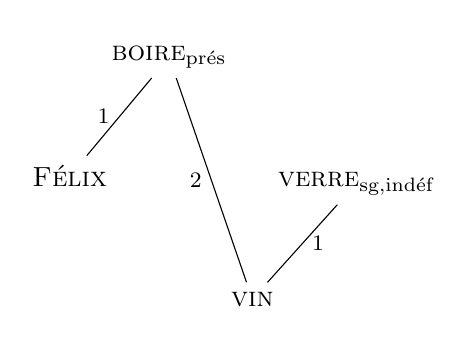
\begin{tikzpicture}[label distance=0pt]
			\matrix (matrix) [nodes={anchor=base},
			ampersand replacement=\&,
			row sep=1cm,
			column sep=-5pt,
			every label/.style={reset shape}] 
			{
				\& \& \node (boire) {\textsc{boire}\textsubscript{prés}}; \& \& \& \\
				\& \node (Felix) {\textsc{Félix}}; \& \& \& \node (verre) {\textsc{verre}\textsubscript{sg,indéf}};\\		
				\& \& \& \node (vin) {\textsc{vin}}; \& \\		
			};
			\draw (boire) -- (Felix) node[font=\footnotesize,midway,left] {1};
			\draw (boire) -- (vin) node[font=\footnotesize,midway,left] {2};
			\draw (verre) -- (vin) node[font=\footnotesize,midway,right] {1};
		\end{tikzpicture}
		\caption{Processus d'insertion}
	\end{subfigure}%
	\hfill
	\begin{subfigure}[b]{0.5\textwidth}
		\centering
		\begin{forest} for tree={font=\normalfont}
			[\textsc{boire}\textsubscript{prés},name=root
			[\textsc{Félix},edge label={node[midway,above left=-0.5ex,font=\footnotesize]{1}}]
			[\ \ \textsc{verre}\textsubscript{sg,indéf},edge label={node[midway,above right=-0.5ex,font=\footnotesize]{(2)}}
			[\textsc{vin},name=vin,edge label={node[midway,right,font=\footnotesize]{1}}]
			]
			]
			\draw[->,dashed] (root) to[out=south,in=west] node[pos=0.75,left]{\footnotesize 2} (vin);
		\end{forest}
		\caption{Structure syntaxique profonde}
	\end{subfigure}
	\caption{Insertion modificative de \REF{ex:13-verre}\label{fig:13-verre}}
\end{figure}

L’insertion modificative concerne aussi les déterminants et en tout premier lieu les dits « déterminants complexes » comme en (\ref{ex:13-insertion})a (voir l’\encadref{sec:3.3.22} sur les \textit{« Déterminants complexes »}). 

\ea\label{ex:13-insertion}
\ea \textit{Félix a lu \textbf{plus de la moitié} du livre.}
\ex \textit{Félix veut acheter \textbf{ce} livre.}\z\z
L’exemple (\ref{ex:13-insertion})a montre de plus que les modifieurs insérés peuvent s’insérer de manière récursive, puisque dans cet exemple \textsc{moitié} vient s’insérer sur \textsc{livre}, puis l’adverbe \textsc{plus} s’insère sur \textsc{moitié}, comme on le voit dans la structure syntaxique profonde de la figure \ref{fig:13-insertion}a. Si l’on considère que les déterminants sont la tête du groupe substantif, comme nous l’avons défendu dans la \sectref{sec:3.3.26} «~\textit{Déterminant comme tête ?}~», alors il faut également considérer que le déterminant \textsc{cet} s’est inséré dans l’exemple (\ref{ex:13-insertion})b. Cette analyse est proposée dans la figure \ref{fig:13-insertion}b et est à contraster avec l’analyse de la figure \ref{fig:13-excellent}, où le nom est considéré comme la tête du groupe substantif et \textsc{cet} est traité comme un modifieur ordinaire.

\begin{figure}
%FIGURE 31
	%a.	Félix <-1- lire\_passé -+-> plus -1-> moitié -1-> livre\_sg, déf <..2.. (lire)
	\begin{subfigure}[b]{0.5\textwidth}
		\centering
		\begin{forest} for tree={font=\normalfont}
			[\textsc{lire}\textsubscript{passé},name=root
			[\textsc{Félix},edge label={node[midway,above left=-0.5ex,font=\footnotesize]{1}}]
			[\textsc{plus},edge label={node[midway,above right=-0.5ex,font=\footnotesize]{(2)}}
			[\textsc{moitié},edge label={node[midway,right,font=\footnotesize]{1}}
			[\textsc{livre}\textsubscript{sg,déf},name=livre,edge label={node[midway,right,font=\footnotesize]{1}}]
			]
			]
			]
			\draw[->,dashed] (root) to[out=south,in=north west] node[pos=0.5,left]{\footnotesize 2} (livre);
		\end{forest}
		\caption{Structure de (\ref{ex:13-insertion})a}
	\end{subfigure}%
	\hfill
	%b.	Félix <-1- vouloir\_prés -2-> acheter -+-> cet -1-> livre\_sg
	% (Félix) <..1..              ..2..> (livre)
	\begin{subfigure}[b]{0.5\textwidth}
		\centering
		\begin{forest} for tree={font=\normalfont}
			[\textsc{vouloir}\textsubscript{prés}
			[\textsc{Félix},name=felix,edge label={node[midway,above left=-0.5ex,font=\footnotesize]{1}}]
			[\textsc{acheter},name=acheter,edge label={node[midway,above right=-0.5ex,font=\footnotesize]{2}}
			[\textsc{cet},edge label={node[midway,right,font=\footnotesize]{(2)}}
			[\textsc{livre}\textsubscript{sg},name=livre,edge label={node[midway,right,font=\footnotesize]{1}}]
			]
			]
			]
			\draw[->,dashed] ($(acheter)+(-0.4cm,-0.4cm)$) .. controls +(south:0.6cm) and +(south:1cm) .. (felix) node[pos=0.5,below]{\footnotesize 1};
			\draw[->,dashed] (acheter) to[out=south east,in=north east] node[pos=0.5,right]{\footnotesize 2} (livre);
		\end{forest}
		\caption{Structure de (\ref{ex:13-insertion})b}
	\end{subfigure}
\caption{Structures syntaxiques profondes de déterminants insérés\label{fig:13-insertion}}
\end{figure}

\section{Les différents types de relations syntaxiques profondes}
En guise de conclusion de ce chapitre, nous souhaitons récapituler les différents types de relations considérées au niveau syntaxique profond. Nous avons au final 6 types de relations syntaxiques profondes à proprement parler :

\begin{itemize}
\item	les relations actancielles, où une relation sémantique et une relation syntaxique se superposent et sont orientées de la même façon ; elles sont étiquetées 1, 2, 3, etc. ou encore ∞ pour un actant rétrogradé ;
\item	les relations modificatives, où une relation sémantique et une relation syntaxique se superposent, mais ont des orientations inverses ; elles sont étiquetées \textit{\textsc{mod}} ;
\item	les relations lexie-grammie, qui sont aussi des cas où une relation sémantique et une relation syntaxique se superposent, mais que nous annotons différemment en raison du statut particulier de la connexion syntaxique entre lexies et grammies ;
\item	les relations entre un opérateur et son argument, que nous utilisons pour la translation syntaxique et pour les sémantèmes cachés ; ces relations généralisent les relations lexie-grammie, puisque les grammies fonctionnent comme des opérateurs prenant la lexie comme argument ;
\item	les relations syntaxiques pures, qui ne se superposent pas à une relation sémantique ; elles sont étiquetées +1, +2, etc., lorsqu'il s'agit de quasi-actants résultant d'une montée, ou (1), (2), etc., lorsqu'il s'agit de positions actancielles où un modifieur s'est inséré ;
\item	les relations sémantiques pures qui ne se superposent pas à une relation syntaxique ; elles sont représentées par des flèches hachurées et sont numérotées comme les relations actancielles.
\end{itemize}

On peut encore ajouter à cette liste deux relations qui appartiennent à la structure référentielle :

\begin{itemize}
\item	les relations de coréférence, qui indiquent la scission d’un nœud sémantique ; elles sont représentées par une flèche bidirectionnelle en pointillés ;
\item	les relations d’ancrage, qui indiquent l’ancrage du référent d’un indéfini sur un autre élément de la structure ou sur l’univers du discours ; elles sont représentées par une flèche en pointillés.
\end{itemize}

D’autres exemples de structures syntaxiques profondes seront donnés dans le \chapfuturef{18} sur les \textit{Listes paradigmatiques} et le \chapfuturef{19} sur l’\textit{Extraction}.

Le volume 1  de \textit{Syntaxe théorique et formelle} se termine ici. Le volume 2 rentrera plus en détail dans la structure syntaxique de surface (sans oublier les structures topologique et syntaxique profonde) en s’intéressant d’abord à la \textit{nanosyntaxe} et à la notion de mot et de catégorie flexionnelle, puis à la \textit{microsyntaxique} et aux catégories lexicales ou parties du discours, aux relation syntaxiques et à deux phénomènes complexes, l’extraction et la coordination, et enfin à la \textit{macrosyntaxe} et à la notion controversée de phrase.\largerpage

\exercices{%
\exercice{1}~(modifieurs \textit{vs} actants)\ \ Pour les compléments de nom suivants, déterminer s’il s’agit d’un actant ou d’un modifieur.
\begin{enumerate}[label=\alph*.]
\item \textit{la réponse de Zoé}
\item \textit{le portrait de Zoé}
\item \textit{la main de Zoé}
\item \textit{la trousse de Zoé}
\item \textit{le chat de Zoé}
\item \textit{une huître de Bretagne}
\item \textit{le phare du Cap Fréhel}
\end{enumerate}


\exercice{2} Reprenons notre exemple de base du \chapref{sec:3.3} :
\begin{exe}
    \exi{} \textit{Beaucoup de gens aimeraient passer Noël en Laponie.}
\end{exe}
Donner la structure prédicative sémantique et la structure syntaxique profonde de cet exemple.



\exercice{3} Pour les exemples suivants, déterminez quels sont les sémantèmes, puis proposez une représentation syntaxique profonde. On notera que ces exemples contiennent un sémantème caché.
\begin{enumerate}[label=\alph*.]
\item \textit{Zoé, faut qu’on y aille !}
\item \textit{Il y a de l’œuf sur ma chemise.}
\end{enumerate}

\exercice{4} On considère la construction suivante :
\begin{exe}
    \exi{} \textit{Je ne comprends rien à ce problème.}
\end{exe}

\begin{enumerate}
\item Montrer que les éléments qui peuvent commuter avec \textit{rien} forme un paradigme très réduit que vous décrirez et tenterez de caractériser.
\item Quel est la contribution sémantique de \textit{rien} dans cette construction ?
\item Bien que \textit{rien} soit réalisé en position d’objet direct, pourquoi peut-on considérer qu’il s’agit d’un modifieur ?
\end{enumerate}

\exercice{5}~(noms temporels)\ \ Quels problèmes posent les noms temporels pour la modélisation ? Comment modéliser les énoncés suivants en syntaxe profonde ?
\begin{enumerate}[label=\alph*.]
\item\textit{Je viendrai la semaine prochaine.}
\item\textit{Il a dormi deux heures.}
\end{enumerate}

\exercice{6} Nous nous intéressons à la construction suivante.
\begin{exe}
\exi{}\textit{Luc casse les œufs dans un bol.}
\end{exe}
\begin{enumerate}
\item Montrer que le complément locatif \textit{dans un bol} n’est pas un modifieur ordinaire indiquant les circonstances du procès.
\item Comment modéliser cette construction ?
\end{enumerate}

\exercice{7} Nous nous intéressons à la construction suivante, appelée \textit{tough-movement} par les générativistes. (Le terme comporte un jeu de mots puisque \textit{tough movement} évoque à la fois un problème épineux qui concerne des adjectifs comme \textit{tough}, qui signifie ‘dur, coriace, épineux’.)
\begin{enumerate}[label=\alph*.]
\item \textit{un livre difficile à lire}
\item\textit{Ce livre est difficile à lire.}
\end{enumerate}
\begin{enumerate}
\item En utilisant la paraphrase avec « \textit{Lire ce livre est difficile} », montrer qu’il s’agit potentiellement d’une construction à montée.
\item Donner la structure prédicative sémantique et la structure syntaxique profonde de ces exemples.
\end{enumerate}

\exercice{8} La synonymie entre les deux phrases suivantes est un peu étrange si on regarde les choses de près.
\begin{enumerate}[label=\alph*.]
\item \textit{On doit dire la vérité.}
\item \textit{On ne doit pas mentir.}
\end{enumerate}
Montrer qu’il y a un apparent phénomène de montée de la négation en jeu.}

\lecturesadditionnelles{La notion de structure syntaxique profonde doit beaucoup aux travaux d’Igor Mel’čuk. Celui-ci a théorisé la notion et a aussi développé des lexiques sémantiques et syntaxiques pour le russe, puis pour le français lorsqu’il a émigré au Québec en 1977. On consultera tout particulièrement son ouvrage de sémantique en 3 volumes (\citeyear{melcuk2012semantics}) et les dictionnaires explicatifs et combinatoires du français (\citeyear{melcuk1999dictionnaire}). Sa modélisation repose de façon essentielle sur la notion d’actant, à laquelle il a consacré de nombreux articles : on retiendra tout particulièrement les deux articles de 2004 \citep{melcuk2004actants1,melcuk2004actants2}.

Le flambeau a été repris par son étudiant, Alain Polguère, dont nous recommandons encore une fois l’ouvrage de sémantique lexicale et lexicologie. Celui-ci développe également un lexique sémantique et syntaxique électronique sous forme de réseau lexical, consultable en ligne sur \url{https://lexical-systems.atilf.fr/spiderlex/}. Dans les travaux de Mel’čuk et Polguère, l’accent est particulièrement mis sur la combinatoire lexicale restreinte décrite à l’aide des fonctions lexicales, dont nous n’avons donné qu’un très faible aperçu dans ce chapitre.

La formalisation de l’interface sémantique sous la forme d’une correspondance entre un graphe sémantique et un arbre de dépendance syntaxique de surface est développée dans le cadre de la Théorie Sens-Texte. La formalisation sous la forme d’une combinaison de structure élémentaire est développée dans les travaux de Sylvain Kahane, dont on pourra consulter le tutoriel sur la Théorie Sens-Texte et les grammaires formelles de \citeyear{kahane2001grammaires} et le mémoire d’habilitation de \citeyear{kahane2002grammaire} consacré à la formalisation de la Théorie Sens-Texte par une grammaire comme celle de l’\encadref{sec:13-derivation}. L’article de \citeyear{kahane2015trois} sur \textit{Les trois dimensions d'une modélisation formelle de la langue} présente une comparaison entre une telle grammaire et les grammaires TAG, avec notamment des exemples de distorsions sémantique-syntaxe.

\FurtherReading{3-6}}

\corrections{%
\corrigé{1} La plupart des compléments de nom considérés sont des actants : \textsc{réponse} est un nom prédicatif dont \textsc{Zoé} est le premier argument ; \textsc{portrait} est un nom prédicatif à deux arguments (quelqu’un fait le portrait de quelqu’un) et \textsc{Zoé} peut être l’un ou l’autre des arguments ; \textsc{main} désigne une partie du corps de quelqu’un ;  \textsc{trousse} désigne un artefact, c’est-à-dire un objet fabriqué pour être utilisé et dont l’utilisateur est donc un argument ; \textsc{chat} désigne un animal domestique, qui à ce titre possède un maître/utilisateur (un animal, lorsqu’il est domestiqué, peut être vu comme une sorte d’artefact). Il est également défendable de considérer \textit{de Zoé} comme un modifieur dans ces deux derniers exemples. On traitera alors la préposition \textsc{de} comme la réalisation d’un sémantème «~possesseur~». Dans les deux derniers exemples, les compléments locatifs \textit{de Bretagne} et \textit{du Cap Fréhel} peuvent être clairement considérés comme des modifieurs. Nous considérons que la préposition \textsc{de} est la réalisation d’un sémantème «~provenance~» dans le premier cas et «~location~» dans le deuxième.

\corrigé{2} Notre exemple de base illustre plusieurs phénomènes intéressants du point de vue de la syntaxe profonde. Deux cas de distorsion sémantique-syntaxe : un verbe à contrôle avec \textsc{aimer} et une insertion modificative avec \textsc{beaucoup}. Notons également que le complément locatif \textit{en Laponie} fait partie de la valence de \textsc{passer} (quelqu’un passe un moment quelque part). Enfin, le nom \textsc{gens} est un nom massif pluriel qui ne varie donc pas en nombre, comme d'ailleurs les noms propres \textsc{Noël} et \textsc{Laponie}. Les représentations sémantique et syntaxique profonde sont données dans la figure \ref{fig:13-laponie}.

\begin{figure}[H]
%FIGURE 32
	%a. ‘beaucoup’ -1-> ‘gens’ <-1- aimer -2-> ‘passer’ -2-> ‘Noël’ 
	%						<..1.. 	-3-> ‘Laponie’
	\begin{subfigure}[h]{\textwidth}
		\centering
		\begin{tikzpicture}[>={Triangle[]},
			label distance=0pt,
			node distance=10mm,
			every label/.style={reset shape}]
			
			\begin{scope}[nodes={CircleNode}]
				\node (beaucoup) [label=above left:{`beaucoup'}] {};
				\node (gens) [below right=of beaucoup,label=below left:{`gens'}] {};
				\node (aimer) [above right=of gens,label=above left:{`aimer'}] {};
				\node (conditionnel) [above right=of aimer,label=above right:{conditionnel}] {};
				\node (passer) [below right=of aimer,label=below left:{`passer'}] {};
				\node (noel) [above right=of passer,label=above right:{`Noël'}] {};
				\node (laponie) [below right=of passer,label=below right:{`Laponie'}] {};
			\end{scope}
			
			\draw[-{Triangle[]}] (beaucoup) -- (gens) node[font=\footnotesize,midway,anchor=base west] {1};
			\draw[-{Triangle[]}] (aimer) -- (gens) node[font=\footnotesize,midway,anchor=base east] {1};
			\draw[-{Triangle[]}] (conditionnel) -- (aimer) node[font=\footnotesize,midway,anchor=base east] {1};
			\draw[-{Triangle[]}] (aimer) -- (passer) node[font=\footnotesize,midway,anchor=base west] {2};
			\draw[-{Triangle[]}] (passer) -- (gens) node[font=\footnotesize,midway,above] {1};
			\draw[-{Triangle[]}] (passer) -- (noel) node[font=\footnotesize,midway,anchor=base east] {2};
			\draw[-{Triangle[]}] (passer) -- (laponie) node[font=\footnotesize,midway,anchor=base west] {3};
			
		\end{tikzpicture}
		\caption{Structure prédicative sémantique}
	\end{subfigure}%
	\bigskip\medskip\\%
	%b. gens\_indf <-1- beaucoup <-+- aimer\_cond -2-> passer Noël Laponie
	\begin{subfigure}[h]{\textwidth}
		\centering
		\begin{forest} for tree={font=\normalfont}
			[\textsc{aimer}\textsubscript{cond},name=root
			[\textsc{beaucoup},edge label={node[midway,above left=-0.5ex,font=\footnotesize]{(1)}}
			[\textsc{gens}\textsubscript{déf},name=gens,edge label={node[midway,left,font=\footnotesize]{1}}]
			]
			[\textsc{passer},name=passer,edge label={node[midway,above right=-0.5ex,font=\footnotesize]{2}}
			[\textsc{Noël},edge label={node[midway,below right,font=\footnotesize]{2}}]
			[\textsc{Laponie},edge label={node[midway,above right=-0.5ex,font=\footnotesize]{3}}]
			]
			]
			\draw[->,dashed] (root) to[out=south,in=north east] node[pos=0.5,right]{\footnotesize 1} (gens);
			\draw[->,dashed] (passer) to[out=south west,in=north east] node[pos=0.25,above]{\footnotesize 1} ($(gens)+(0.75,0.25)$);
		\end{forest}
		\caption{Structure syntaxique profonde}
	\end{subfigure}
\caption{Structures pour notre phrase préférée\label{fig:13-laponie}}
\end{figure}

\corrigé{3}
\begin{enumerate}[label=\alph*.]
    \item Le vocatif \textit{Zoé} contient un sémantème caché. Il ne s’agit pas vraiment d’un dépendant de la construction verbale \textit{faut qu’on y aille}, mais d’un élément qui se rattache directement à l’illocution et peut être paraphrasé par ‘je déclare à Zoé qu’il faut qu’on y aille’ (voir la figure \ref{fig:13-vocatif}a). Cet élément de sens n’étant pas lexicalisé, nous le traitons comme un sémantème caché « vocatif ». Par ailleurs, nous traitons \phraseme{y aller} comme un phrasème, car dans cette expression \textsc{y} n’est pas a priori un pronom anaphorique correspondant à une destination précise. Enfin, le subjonctif sur ce verbe est imposé par le verbe \textsc{falloir} et n’est donc pas un sémantème.
    
\begin{figure}[H]
%Figure 33 
	%a.	‘Zoé’ <-2- déclaration -1-> ‘falloir’ -1-> ‘y aller’ -1-> ‘on’
	\begin{subfigure}[b]{.5\linewidth}%
		\centering%
		\begin{tikzpicture}[>={Triangle[]},
			label distance=0pt,
			node distance=10mm and 10mm,
			every label/.style={reset shape,font=\strut}]
			
			\begin{scope}[nodes={CircleNode}]
				\node (moi) [label=below:{`moi'}] {};
				\node (declarer) [above right=of moi,label=above:{`déclarer'}] {};
				\node (zoe) [below=9.333mm of declarer,label=below:{`Zoé'}] {};
				\node (falloir) [below right=of declarer,label=below:{`falloir'}] {};
				\node (yaller) [above right=of falloir,label=above:{`y aller'}] {};
				\node (on) [below right=of yaller,label=below:{`on'}] {};
			\end{scope}
			\draw[-{Triangle[]}] (declarer) -- (moi) node[font=\footnotesize,midway,left] {1};
			\draw[-{Triangle[]}] (declarer) -- (zoe) node[font=\footnotesize,midway,right] {3};
			\draw[-{Triangle[]}] (declarer) -- (falloir) node[font=\footnotesize,midway,right] {2};
			\draw[-{Triangle[]}] (falloir) -- (yaller) node[font=\footnotesize,midway,right] {1};
			\draw[-{Triangle[]}] (yaller) -- (on) node[font=\footnotesize,midway,right] {1};
		\end{tikzpicture}
		\caption{Structure prédicative sémantique}
	\end{subfigure}%
	%b.	vocatif(Zoé) <-MOD- falloir\_présent -1-> \phraseme{y aller} -1-> on
	\begin{subfigure}[b]{.5\linewidth}
		\centering
		\begin{forest} for tree={font=\normalfont}
			[\textsc{falloir}\textsubscript{présent}
			[vocatif(\textsc{Zoé}),edge label={node[midway,above left=-0.5ex,font=\footnotesize\itshape]{\textsc{mod}}}]
			[\phraseme{y aller},edge label={node[midway,above right=-0.5ex,font=\footnotesize]{1}}
			[\textsc{on},edge label={node[midway,right,font=\footnotesize]{1}}]
			]
			]
		\end{forest}
		\caption{Structure syntaxique profonde}
	\end{subfigure}%
\caption{Structures pour un vocatif\label{fig:13-vocatif}}
\end{figure}

\item Le nom \textsc{œuf} est un nom comptable. Il est employé ici comme un massif, avec le déterminant indéfini des massifs (qu'on appelle traditionnellement le \hi{partitif}). Nous considérons donc qu’il est combiné avec un sémantème caché « massif », qui signifie ‘une matière formée de’. Ce sémantème joue le rôle inverse du sémantème «~type~», qui produit un nom comptable à partir d’un massif. Par ailleurs, nous traitons \textit{il y a} comme la réalisation d’un phrasème \phraseme{il y avoir} qui « verbalise » la préposition \textsc{sur}. Enfin, nous traitons le possesif \textit{ma} comme un modifieur obtenu par la combinaison du pronom \textsc{moi} avec le sémantème «~possesseur~», qui peut être réalisé par la préposition \textsc{de} (voir le corrigé de l’exercice 1) ou par un grammème comme ici.

\begin{figure}[H]
%Figure 34
%massif(œuf)\_indéf <-1- \phraseme{il y avoir}\_présent -2-> sur -2-> chemise\_déf -MOD-> possessif(moi)
%							(œuf) <..1..
\begin{forest} for tree={font=\normalfont}
	[\phraseme{il y avoir}\textsubscript{prés}
	[massif(\textsc{œuf})\textsubscript{indéf},name=oeuf,edge label={node[midway,above left=-0.5ex,font=\footnotesize]{1}}]
	[\textsc{sur}, name=sur,edge label={node[midway,above right=-0.5ex,font=\footnotesize]{2}}
	[\textsc{chemise},edge label={node[midway,right,font=\footnotesize]{2}}
	[possesseur(\textsc{moi}),edge label={node[midway,right,font=\footnotesize\itshape]{\textsc{mod}}}]
	]
	]
	]
	\draw[->,dashed] ($(sur)+(-0.125cm,-0.4cm)$) .. controls +(south:0.8cm) and +(south:1.2cm) .. (oeuf) node[pos=0.5,below left]{\footnotesize 1};
\end{forest}
\caption{Structure syntaxique profonde d'une conversion comptable-massif}
\end{figure}
\end{enumerate}

\pagebreak\corrigé{4} Nous avons déjà présenté cette unité lexicale étrange dans l’\encadref{sec:0.0.7} intitulé \textit{Le lexique : un cabinet de curiosités}. Le paradigme de commutation de \textit{rien} comprend uniquement \textit{quelque chose}, \textit{pas grand-chose}, \textit{que dalle} et les formes interrogatives \textit{que/quoi} et \textit{qu'est-ce que}. Nous considérons donc que ce paradigme forme un phrasème avec le verbe \textsc{comprendre}, phrasème que nous proposons d’appeler \phraseme{comprendre quelque chose}. Ce phrasème doit obligatoirement se combiner avec une négation ou une interrogation et le complément \textsc{rien}, qui est la négation de \textsc{quelque chose}, porte donc juste la valeur négative : négation + \phraseme{comprendre quelque chose} =  \textit{ne rien comprendre}. Cette valeur négative fonctionne comme un modifieur. 


\corrigé{5} Les noms temporels indiquent un moment (\textit{la semaine prochaine}) ou une durée (\textit{deux heures}). Dans les exemples donnés, ils sont utilisés comme des modifieurs de verbes. En même temps, ce sont de vrais noms, qui peuvent être utilisés, avec le même sens exactement, dans des positions où on attend un substantif : \textit{\textbf{deux heures} suffiront pour terminer} \textit{la réunion de \textbf{la semaine prochaine}}. Nous considérons donc qu’il y a des sémantèmes cachés qui se combinent avec les noms temporels et permettent de les utiliser comme modifieurs. Nous nommons ces sémantèmes « moment » et « durée ». On notera que ces sémantèmes sont bi-valents : leur premier argument est le verbe et leur deuxième argument le nom temporel.

\begin{figure}[H]
%FIGURE 35
	%a. moi venir\_futur moment(semaine\_def) prochain
	\begin{subfigure}[b]{0.5\textwidth}
		\centering
		\begin{forest} for tree={font=\normalfont}
			[\textsc{venir}\textsubscript{futur}
			[\textsc{moi},edge label={node[midway,above left=-0.5ex,font=\footnotesize]{1}}]
			[moment(\textsc{semaine}\textsubscript{sg,def}),edge label={node[midway,above right=-0.5ex,font=\footnotesize\itshape]{\textsc{mod}}}
			[\textsc{prochain},edge label={node[midway,right,font=\footnotesize\itshape]{\textsc{mod}}}]
			]
			]
		\end{forest}
		\caption{Structure pour un moment}
	\end{subfigure}%
	\hfill
	%b. lui dormir\_passé durée(heure\_indf) deux
	\begin{subfigure}[b]{0.5\textwidth}
		\centering
		\begin{forest} for tree={font=\normalfont}
			[\textsc{dormir}\textsubscript{passé}
			[\textsc{lui},edge label={node[midway,above left=-0.5ex,font=\footnotesize]{1}}]
			[durée(\textsc{heure}\textsubscript{pl,indéf}),edge label={node[midway,above right=-0.5ex,font=\footnotesize\itshape]{\textsc{mod}}}
			[\textsc{deux},edge label={node[midway,right,font=\footnotesize\itshape]{\textsc{mod}}}]
			]
			]
		\end{forest}
		\caption{Structure pour une durée}
	\end{subfigure}
\caption{Structures syntaxiques profondes de noms temporels modifieurs}
\end{figure}

\corrigé{6} Lorsque Luc casse des œufs, le procès n’a pas lieu dans un bol : le bol est la destination des œufs. Le verbe \textsc{casser} a ici le sens habituel ‘casser’, mais la construction de \textsc{mettre} (\textit{Luc met les œufs dans un bol}). On peut donc imaginer plusieurs modélisations possibles. Si l’on traite \textit{dans un bol} comme un modifieur, il y a nécessairement un sémantème caché indiquant qu’il s’agit d’une destination. Ce sémantème, que nous nommons « destination », est une façon d’indiquer que la construction est signifiante. On peut aussi considérer que ce complément est « entré » dans la valence du verbe \textsc{casser} et qu’on a une acception trivalente de ce verbe, un \textsc{casser}\textsubscript{b}, équivalent au \textsc{casser}\textsubscript{a} + destination. Cette construction, plus courante en anglais qu'en français, a été appelée la \hi{construction résultative}. On pourra notamment consulter le livre d'Adele \citet{goldberg1995constructions} qui y consacre un chapitre.

\begin{figure}[H]
%FIGURE 36
	%a.
	\begin{subfigure}[b]{0.5\textwidth}
		\centering
		\begin{forest} for tree={font=\normalfont}
			[\textsc{casser}\textsubscript{prés}, calign=child, calign primary child=2
			[\textsc{Zoé},edge label={node[midway,above left,font=\footnotesize]{1}}]
			[\textsc{œuf}\textsubscript{pl,déf},edge label={node[midway,right,font=\footnotesize]{2}}]
			[destination(\textsc{dans}),edge label={node[midway,above right,font=\footnotesize\itshape]{\textsc{mod}}}
			[\textsc{bol}\textsubscript{sg,déf},edge label={node[midway,right,font=\footnotesize]{2}}]
			]
			]
		\end{forest}
		\caption{Traitement comme modifieur}
	\end{subfigure}%
	\hfill
	%b.
	\begin{subfigure}[b]{0.5\textwidth}
		\centering
		\begin{forest} for tree={font=\normalfont}
			[\textsc{casser}\textsubscript{prés}, calign=child, calign primary child=2
			[\textsc{Zoé},edge label={node[midway,above left,font=\footnotesize]{1}}]
			[\textsc{œuf}\textsubscript{pl,déf},edge label={node[midway,right,font=\footnotesize]{2}}]
			[\textsc{dans},edge label={node[midway,above right,font=\footnotesize]{3}}
			[\textsc{bol}\textsubscript{sg,déf},edge label={node[midway,right,font=\footnotesize]{2}}]
			]
			]
		\end{forest}
		\caption{Traitement comme actant}
	\end{subfigure}
\caption{Deux structures syntaxiques syntaxiques possibles pour une construction résultative}
\end{figure}

\corrigé{7} Si l’on accepte la paraphrase entre « \textit{Ce livre est difficile à lire.}~» et « \textit{Lire ce livre est difficile} », alors on peut considérer que \textsc{difficile} reste un prédicat à un argument dans la construction dite du «~tough-movement~» (voir la structure prédicative de la figure \ref{fig:13-tough}c). Dans cette construction, l'adjectif a néanmoins deux actants en raison de la montée du deuxième argument de \textsc{lire} en position de premier actant de \textsc{difficile}, tandis que le premier argument de \textsc{lire} est rétrogradé en position de deuxième actant. Comme il existe plusieurs adjectifs qui ont les deux constructions (\textsc{facile}, \textsc{impossible}, \textsc{utile} …), nous considérerons, à la suite des générativistes, qu’il s’agit d’une réorganisation de la valence de l’adjectif (plutôt que de deux acceptions du même adjectif). Dans notre cadre, une telle réorganisation résulte de la combinaison avec un sémantème constructionnel, que nous appellerons «~{tough-movement}~» (pour ne pas rompre avec la tradition). Il en résulte les structures syntaxiques profondes des figures \ref{fig:13-tough}a et b.

\begin{figure}[H]
%FIGURE 37\label{fig:13-tough}
	%a. livre\_sg, indf -+-> tough-mvt(difficile) -1-> lire\_inf
	\begin{subfigure}[b]{0.5\textwidth}
		\centering
		\begin{forest} for tree={font=\normalfont}
			[\textsc{livre}\textsubscript{sg,indéf},name=root
			[tough-mvt(\textsc{difficile}),name=mvt,edge label={node[midway,right,font=\footnotesize]{+\textsc{mod}}}
			[\textsc{lire}\textsubscript{inf},name=lire,edge label={node[midway,right,font=\footnotesize]{2}}]%
			]
			]
			\draw[->,dashed] (lire) .. controls +(west:3cm) and +(west:3cm) .. (root) node[pos=0.5, left]{\footnotesize 2};
		\end{forest}
		\caption{Structure syntaxique profonde de a}
	\end{subfigure}%
	\hfill
	%b. V(tough-mvt(difficile))\_prés …
	\begin{subfigure}[b]{0.5\textwidth}
		\centering
		\begin{forest} for tree={font=\normalfont}
			[V(tough-mvt(\textsc{difficile}))\textsubscript{prés}
			[\textsc{livre}\textsubscript{sg},name=livre,edge label={node[midway,above left=-0.5ex,font=\footnotesize]{+1}}
			[\textsc{cet},edge label={node[midway,left,font=\footnotesize\itshape]{\textsc{mod}}}]
			]
			[\textsc{lire}\textsubscript{inf},name=lire,edge label={node[midway,above right=-0.5ex,font=\footnotesize]{2}}]
			]
			\draw[->,dashed] ($(lire)+(-0.125cm,-0.4cm)$) .. controls +(south:0.6cm) and +(south:0.8cm) .. ($(livre)+(0.25cm,-0.4cm)$) node[pos=0.5,below]{\footnotesize 2};
		\end{forest}
		\caption{Structure syntaxique profonde de b}
	\end{subfigure}%
	\bigskip\\%
	%c. ‘difficile’ -1-> ‘lire’ -1-> ‘livre’
	\begin{subfigure}[h]{\textwidth}
		\centering
		\begin{tikzpicture}[>={Triangle[]},
			label distance=0pt,
			node distance=10mm,
			every label/.style={reset shape}]
			
			\begin{scope}[nodes={CircleNode}]
				\node (generique) [label=below:{générique}] {};
				\node (lire) [above right=of generique,label=above left:{`lire'}] {};
				\node (difficile) [right=of lire,label=right:{`difficile'}] {};
				\node (livre) [below right=of lire,label=below:{`livre'}] {};
			\end{scope}
			
			\draw[-{Triangle[]}] (lire) -- (generique) node[font=\footnotesize,midway,anchor=base east] {1};
			\draw[-{Triangle[]}] (lire) -- (livre) node[font=\footnotesize,midway,anchor=base west] {2};
			\draw[-{Triangle[]}] (difficile) -- (lire) node[font=\footnotesize,midway,above] {1};
			
		\end{tikzpicture}
		\caption{Structure prédicative commune}
	\end{subfigure}
\caption{Structures pour le tough-movement\label{fig:13-tough}}
\end{figure}

\corrigé{8} « \textit{On ne doit pas mentir.} » ne signifie pas ‘il est faux qu'on doit mentir’ et
n’est donc pas la négation sémantique de «~\textit{On doit mentir.}~». Celle-ci serait plutôt exprimée par «~\textit{On n’est pas obligé de mentir.}~» ou «~\textit{On peut ne pas mentir.}~». En fait, «~\textit{On ne doit pas mentir.}~» est synonyme de «~\textit{On doit ne pas mentir.}~». Il y a donc bien un apparent phénomène de montée de la négation : la négation qui porte sémantiquement sur \textsc{mentir} se trouve attachée syntaxiquement au verbe recteur \textsc{devoir}. \citet{tesniere1959elements} notait déjà ce phénomène auquel il consacre son chapitre 89 intitulé \textit{Anticipation de la négation}. Plutôt qu’un phénomène syntaxique qui verrait véritablement une montée dans l’interface sémantique-syntaxe, il s’agit plus sûrement d’un phénomène de figement lexical associé au verbe recteur, qui, combiné à la négation, prend un sens particulier (voir par exemple \citealt{forest1994negation}). On retrouve ce phénomène dans de nombreuses langues. Cet exemple de l’italien montre un contraste intéressant avec le français :

\begin{exe}
\exi{} \textit{Il caffè non mi fa dormire.}\\
‘Le café m’empêche de dormir.’\\
litt. Le café ne me fait pas dormir.
\end{exe}
A l'inverse, le verbe \textsc{müssen} qui est l'équivalent de \textsc{devoir} en allemand ne présente pas de figement avec la négation :

\begin{exe}
\exi{} \textit{Man muss nicht die Wahrheit sagen.}\\
'On n'est pas obligé de dire la vérité.'\\
litt. On ne doit pas dire la vérité.
\end{exe}}

